\documentclass[a4paper,fleqn,usenatbib]{mnras}

\usepackage{ae, aecompl, amsmath, amssymb}
\usepackage{bm}           %%  bold math
\usepackage{cancel, mathptmx}
\usepackage{color}
\usepackage{dcolumn}  %%  Align table columns on decimal point
\usepackage{epsfig, epsf, etoolbox}
\usepackage{fancyhdr}
\usepackage{graphicx}
\usepackage[T1]{fontenc}
%\usepackage{lscape}
\usepackage{ifthen}
\usepackage{hyperref}
\usepackage{listings}
\usepackage{longtable}
\usepackage{multirow}
\usepackage{newtxtext, newtxmath}
\usepackage{pifont}% http://ctan.org/pkg/pifont
\usepackage{subfigure}
\usepackage{tabu}

\usepackage{verbatim}

\usepackage{xcolor}
%\usepackage[square, sort, comma, numbers]{natbib}
\usepackage{threeparttable}
%\usepackage[square,sort,comma,numbers]{natbib}

\usepackage{graphicx}	% Including figure files
\usepackage{tikz}
\def\checkmark{\tikz\fill[scale=0.4](0,.35) -- (.25,0) -- (1,.7) -- (.25,.15) -- cycle;} 

%%  I dont know why, but arydshln leads to pdflatex crashing (when using 'regular' hline)
%% if you load this package at the top of this list.  e.g. 
%%    tex.stackexchange.com/questions/419497/hline-doesnt-compile-arydshln-and-tabularx-incompatibility
\usepackage{arydshln}


%%%%%%%%%%%%%%%%%%%%%%%%%%%%%%%%%%%%%%%%%%%
%       define Journal abbreviations      %
%%%%%%%%%%%%%%%%%%%%%%%%%%%%%%%%%%%%%%%%%%%
\def\nat{Nat} \def\apjl{ApJ~Lett.} \def\apj{ApJ}
\def\apjs{ApJS} \def\aj{AJ} \def\mnras{MNRAS}
\def\prd{Phys.~Rev.~D} \def\prl{Phys.~Rev.~Lett.}
\def\plb{Phys.~Lett.~B} \def\jhep{JHEP}
\def\npbps{NUC.~Phys.~B~Proc.~Suppl.} \def\prep{Phys.~Rep.}
\def\pasp{PASP} \def\aap{Astron.~\&~Astrophys.} \def\araa{ARA\&A}
\def\jcap{\ref@jnl{J. Cosmology Astropart. Phys.}} 
\def\nar{New~A.R.} 

\newcommand{\preep}[1]{{\tt #1} }

%%%%%%%%%%%%%%%%%%%%%%%%%%%%%%%%%%%%%%%%%%%%%%%%%%%%%
%              define symbols                       %
%%%%%%%%%%%%%%%%%%%%%%%%%%%%%%%%%%%%%%%%%%%%%%%%%%%%%
\def \Mpc {~{\rm Mpc} }
\def \Om {\Omega_0}
\def \Omb {\Omega_{\rm b}}
\def \Omcdm {\Omega_{\rm CDM}}
\def \Omlam {\Omega_{\Lambda}}
\def \Omm {\Omega_{\rm m}}
\def \ho {H_0}
\def \qo {q_0}
\def \lo {\lambda_0}
\def \kms {{\rm ~km~s}^{-1}}
\def \kmsmpc {{\rm ~km~s}^{-1}~{\rm Mpc}^{-1}}
\def \hmpc{~\;h^{-1}~{\rm Mpc}} 
\def \hkpc{\;h^{-1}{\rm kpc}} 
\def \hmpcb{h^{-1}{\rm Mpc}}
\def \dif {{\rm d}}
\def \mlim {m_{\rm l}}
\def \bj {b_{\rm J}}
\def \mb {M_{\rm b_{\rm J}}}
\def \mg {M_{\rm g}}
\def \mi {M_{\rm i}}
\def \qso {_{\rm QSO}}
\def \lrg {_{\rm LRG}}
\def \gal {_{\rm gal}}
\def \xibar {\bar{\xi}}
\def \xis{\xi(s)}
\def \xisp{\xi(\sigma, \pi)}
\def \Xisig{\Xi(\sigma)}
\def \xir{\xi(r)}
\def \max {_{\rm max}}
\def \gsim { \lower .75ex \hbox{$\sim$} \llap{\raise .27ex \hbox{$>$}} }
\def \lsim { \lower .75ex \hbox{$\sim$} \llap{\raise .27ex \hbox{$<$}} }
\def \deg {^{\circ}}
%\def \sqdeg {\rm deg^{-2}}
\def \deltac {\delta_{\rm c}}
\def \mmin {M_{\rm min}}
\def \mbh  {M_{\rm BH}}
\def \mdh  {M_{\rm DH}}
\def \msun {M_{\odot}}
\def \z {_{\rm z}}
\def \edd {_{\rm Edd}}
\def \lin {_{\rm lin}}
\def \nonlin {_{\rm non-lin}}
\def \wrms {\langle w_{\rm z}^2\rangle^{1/2}}
\def \dc {\delta_{\rm c}}
\def \wp {w_{p}(\sigma)}
\def \PwrSp {\mathcal{P}(k)}
\def \DelSq {$\Delta^{2}(k)$}
\def \WMAP {{\it WMAP \,}}
\def \cobe {{\it COBE }}
\def \COBE {{\it COBE \;}}
\def \HST  {{\it HST \,\,}}
\def \Spitzer  {{\it Spitzer \,}}
\def \ATLAS {VST-AA$\Omega$ {\it ATLAS} }
\def \BEST   {{\tt best} }
\def \TARGET {{\tt target} }
\def \TQSO   {{\tt TARGET\_QSO}}
\def \HIZ    {{\tt TARGET\_HIZ}}
\def \FIRST  {{\tt TARGET\_FIRST}}
\def \zc {z_{\rm c}}
\def \zcz {z_{\rm c,0}}


\newcommand{\sqdeg}{deg$^{-2}$}
\newcommand{\lya}{Ly$\alpha$\ }
%\newcommand{\lya}{Ly\,$\alpha$\ }
\newcommand{\lyaf}{Ly\,$\alpha$\ forest}
%\newcommand{\eg}{e.g.~}
%\newcommand{\etal}{et~al.~}
\newcommand{\cii}{C\,{\sc ii}\ }
\newcommand{\ciii}{C\,{\sc iii}]\ }
\newcommand{\civ}{C\,{\sc iv}}
\newcommand{\siiv}{Si\,{\sc iv}\ }
\newcommand{\mgii}{Mg\,{\sc ii}\ }
\newcommand{\feii}{Fe\,{\sc ii}\ }
\newcommand{\feiii}{Fe\,{\sc iii}\ }
\newcommand{\caii}{Ca\,{\sc ii}\ }
\newcommand{\halpha}{H\,$\alpha$\ }
\newcommand{\hbeta}{H\,$\beta$\ }
\newcommand{\oi}{[O\,{\sc i}]\ }
\newcommand{\oii}{[O\,{\sc ii}]\ }
\newcommand{\oiii}{[O\,{\sc iii}]\ }
\newcommand{\heii}{[He\,{\sc ii}]\ }
\newcommand{\nii}{N\,{\sc ii}\ }
\newcommand{\nv}{N\,{\sc v}\ }

%% From:: /cos_pc19a_npr/LaTeX/proposals/JWST/JWST_ERS/Proposal/lines.tex
%%  
\newcommand{\imw}{$i$--$W3$}
\newcommand{\imwf}{$i$--$W4$}
\newcommand{\rmwf}{$r$--$W4$}
\newcommand{\imwt}{$i$--$W2$}
\newcommand{\wtmwf}{$W3$--$W4$}
%\newcommand{\kms}{km s$^{-1}$}
\newcommand{\cmN}{cm$^{-2}$}
\newcommand{\cmn}{cm$^{-3}$}
%\newcommand{\msun}{M$_{\odot}$}
\newcommand{\lsun}{L$_{\odot}$}
\newcommand{\lam}{$\lambda$}
\newcommand{\mum}{$\mu$m}
\newcommand{\ebv}{$E(B$$-$$V)$}
%\newcommand{\heii}{\mbox{He\,{\sc ii}}}
\newcommand{\cv}{\mbox{C\,{\sc v}}}
%\newcommand{\civ}{\mbox{C\,{\sc iv}}}
%\newcommand{\ciii}{\mbox{C\,{\sc iii}}}
%\newcommand{\cii}{\mbox{C\,{\sc ii}}}
%\newcommand{\nv}{\mbox{N\,{\sc v}}}
\newcommand{\niv}{\mbox{N\,{\sc iv}}}
\newcommand{\niii}{\mbox{N\,{\sc iii}}}
%\newcommand{\oi}{\mbox{O\,{\sc i}}}
%\newcommand{\oii}{\mbox{O\,{\sc ii}}}
%\newcommand{\oiii}{\mbox{[O\,{\sc iii}]}}
\newcommand{\oiv}{\mbox{O\,{\sc iv}}}
\newcommand{\ov}{\mbox{O\,{\sc v}}}
\newcommand{\ovi}{\mbox{O\,{\sc vi}}}
\newcommand{\ovii}{\mbox{O\,{\sc vii}}}

%\newcommand{\feii}{\mbox{Fe\,{\sc ii}}}
%\newcommand{\feiii}{\mbox{Fe\,{\sc iii}}}
%\newcommand{\mgii}{\mbox{Mg\,{\sc ii}}}
\newcommand{\neii}{[Ne\,{\sc ii}]\ }
\newcommand{\neiii}{[Ne\,{\sc ii}]\ }
\newcommand{\nev}{Ne\,{\sc v}\ }
\newcommand{\nevi}{[Ne\,{\sc vi}]\ }
\newcommand{\neviii}{\mbox{Ne\,{\sc viii}}}
\newcommand{\aliii}{\mbox{Al\,{\sc iii}}}
\newcommand{\siii}{\mbox{Si\,{\sc ii}}}
\newcommand{\siiii}{\mbox{Si\,{\sc iii}}}
%\newcommand{\siiv}{\mbox{Si\,{\sc iv}}}
%\newcommand{\lya}{\mbox{Ly$\alpha$}}
%\newcommand{\lyb}{\mbox{Ly$\beta$}}
\newcommand{\hi}{\mbox{H\,{\sc i}}}
\newcommand{\snine}{\mbox{[S\,{\sc ix}]}}
\newcommand{\sivi}{\mbox{[Si\,{\sc vi}]}}
\newcommand{\sivii}{\mbox[{Si\,{\sc vii}]}}
\newcommand{\siix}{\mbox{[Si\,{\sc ix}]}}
\newcommand{\six}{\mbox{[Si\,{\sc x}]}}
\newcommand{\sixi}{\mbox{[Si\,{\sc xi}]}}
\newcommand{\caviii}{\mbox{[Ca\,{\sc viii}]}}
\newcommand{\arii}{\mbox{[Ar\,{\sc ii}]}}

%%[Ar II] 6.97
%% [S IX] 1.252 μm 328 
% [Si X] 1.430 μm 351 
% [Si XI] 1.932 μm 401 
% [Si VI] 1.962 μm 167 
% [Ca VIII] 2.321 μm 128 
% [Si VII] 2.483 μm 205 
% [Si IX] 3.935 μm 303
% [Ar II] 6.97


%\snine\ at 1.252$\mu$m, \six\ at 1.430$\mu$m, \sixi\ at 1.932$\mu$m, \sivi\ at
%1.962$\mu$m, \caviii\ at 2.321$\mu$m, \sivi\ at 2.483$\mu$m \siix\ at
%3.935$\mu$m and \arii\ at 6.97$\mu$m. 
%%
%% such as [Ne ii]12.8 μm, [Ne v]14.3 μm, [Ne iii]15.5 μm, [S iii]18.7 μm and 33.48 μm, [O iv]25.89 μm and [Si ii]34.8 μm (e.g
%%
%% MIR emission lines like [NeII] and [NeV] are ..
%%
%% Also,  arXiv:astro-ph/0003457v1 
%% [NeV] 14.32um & 24.32um and [NeVI] 7.65um imply an A(V)>160 towards the NLR...
%% [NeIII]15.56um/[NeII]12.81um
%%
%% [Ne V] 14.3, 24.2 μm 97.
%% [Ne II] 12.8 μm
%% [OIV] 26μm
%%


%%%%%%%%%%%%%%%%%%%%%%%%%%%%%%%%%%%%%%%%%%%%%%%%%%%%%
%              define Listings                       %
%%%%%%%%%%%%%%%%%%%%%%%%%%%%%%%%%%%%%%%%%%%%%%%%%%%%%
\definecolor{dkgreen}{rgb}{0,0.6,0}
\definecolor{gray}{rgb}{0.5,0.5,0.5}
\definecolor{mauve}{rgb}{0.58,0,0.82}

\lstset{frame=tb,
  language=Python,
  aboveskip=3mm,
  belowskip=3mm,
  showstringspaces=false,
  columns=flexible,
  basicstyle={\small\ttfamily},
  numbers=none,
  numberstyle=\tiny\color{gray},
  keywordstyle=\color{blue},
  commentstyle=\color{dkgreen},
  stringstyle=\color{mauve},
  breaklines=true,
  breakatwhitespace=true,
  tabsize=3
}

\title[High-redshift CLQs]{The first high-redshift Changing Look Quasars}

\author[Bercow]
{The RH John~S.~Bercow, MP, {\it et al.} 
  % Nicholas~P.~Ross$^{1}$\thanks{E-mail: npross@roe.ac.uk},
  %Matthew Graham$^{2}$, K. E. Saavik Ford$^{3,4,5}$,    Barry McKernan$^{3,4,5}$,  
%\newauthor Daniel Stern$^{6}$, 
\\
% List of institutions
$^{1}$Speaker's Chair, The House of Commons, London, SW1A 0AA \\
%$^{1}$Institute for Astronomy, University of Edinburgh, Royal Observatory, Blackford Hill, Edinburgh EH9 3HJ, United Kingdom \\
%$^{2}$Cahill Center for Astronomy and Astrophysics, California Institute of Technology, Mail Code 249/17, 1200 E California Blvd, Pasadena CA 91125, USA\\
%$^{3}$Department of Science, BMCC, City University of New York, New York, NY 10007, USA \\
%$^{4}$Department of Astrophysics, Rose Center for Earth and Space, American Museum of Natural History, Central Park West at 79th Street, NY 10024, USA \\
%$^{5}$Graduate Center, City University of New York, 365 5th Avenue, New York, NY 10016, USA\\
%$^{6}$Jet Propulsion Laboratory, California Institute of Technology, 4800 Oak Grove Drive, Mail Stop 169-221, Pasadena, CA 91109, USA \\
}

\date{Accepted XXX. Received YYY; in original form ZZZ}
\pubyear{2018}

\hypersetup{draft}

\begin{document}
\label{firstpage}
\pagerange{\pageref{firstpage}--\pageref{lastpage}}
\maketitle

\begin{abstract}
We report on three redshift $z>2$ quasars with dramatic changes in
their \civ\ emission lines, the first `Changing-Look'' quasars at high
redshift.  This is also the first time the changing-look behaviour has
been seen in a high-ionization emission line.
%%
SDSS J1205+3422, J1638+2827 and J2228+2201 show interesting behaviour
in their observed optical light curves, and subsequent spectroscopy
shows significant changes in the \civ\ broad emission line, with both
line collapse and emergence being displayed in rest-frame timescales
of $\sim$240-1640 days.
%%
Where observed, the profile of the Ly$\alpha$/\nv emission complex
also changes, and there is tentative evidence for changes in the \mgii
line.
%%
Although line measurements from the three quasars show large changes
in the \civ\ line flux-line width plane, the quasars are not seen to
be outliers when considered against the full $z\sim2$ quasar population
in terms of (rest) Equivalent Width and FWHM properties.
%%
We put these observations in context with recent ``state-change''
models, but note that even in their `low-state', the \civ\ CLQs are
above $\sim$10\% in Eddington luminosity.
\end{abstract}



% Select between one and six entries from the list of approved keywords.
% Don't make up new ones.
\begin{keywords}
accretion, accretion discs -- surveys -- quasars: general -- quasars: individual: J1100-0053 
\end{keywords}



%%%%%%%%%%%%%%%%%%%%%%%%%%%%%%%%%%%%%%%%%%%%%%%%%%%%%%%%%%%%%%%%%%%%%%%%%%%%%%%%%
%%%%%%%%%%%%%%%%%%%%%%%%%%%%%%%%%%%%%%%%%%%%%%%%%%%%%%%%%%%%%%%%%%%%%%%%%%%%%%%%%
%%
%%
%%   SECTION 1  SECTION 1  SECTION 1  SECTION 1  SECTION 1  SECTION 1  
%%   SECTION 1  SECTION 1  SECTION 1  SECTION 1  SECTION 1  SECTION 1  
%%   SECTION 1  SECTION 1  SECTION 1  SECTION 1  SECTION 1  SECTION 1  
%%
%%
%%%%%%%%%%%%%%%%%%%%%%%%%%%%%%%%%%%%%%%%%%%%%%%%%%%%%%%%%%%%%%%%%%%%%%%%%%%%%%%%%%
%%%%%%%%%%%%%%%%%%%%%%%%%%%%%%%%%%%%%%%%%%%%%%%%%%%%%%%%%%%%%%%%%%%%%%%%%%%%%%%%%%
\section{Introduction}
Luminous AGN, i.e. quasars, are now seen to significantly vary their
energy output on timescales of weeks to months.  This observation, and
the subsequent mismatch in the expected ``viscous'' timescale, which
for a $\approx$10$^{7}$ M$_{\odot}$ central supermassive black hole
(SMBH) is $\sim$hundreds of years, was noted over 30 years ago
\citep[e.g.][]{Alloin1985}. However, with new photometric light-curve
and repeat spectroscopic data, the desire for a deeper understanding
of AGN accretion disk physics has been recently re-invigorated the
field \citep[e.g.][]{Lawrence2018, Antonucci2018}.

The optical continuum variability of quasars has been recognized since
their first optical identification
\citep[e.g.,][]{MatthewsSandage1963, MacLeod2012}.  Dramatic changes
in the broad emission lines (BELs) of quasars has only recently been
identified \citep[e.g., ][]{LaMassa2015}.  Samples of over 100
``Changing Look'' quasars (CLQs) or ``Changing State'' quasars (CSQs)
have now been assembled \citep[e.g.][]{MacLeod2019,Graham2019}. The
community uses both these terms as a cover for the underlying
physics. For sake of argument, ``Changing Look'' quasars can
potentially be thought of as the extension to the BELs of quasar
continuum variability \citep[e.g., ][]{MacLeod2012} whereas the
``Changing State'' quasars (CSQs) have a `state-transition' similar to
that in Galactic X-ray binaries \citep[][]{NodaDone2018, Ruan2019}. In
this paper, we use the term `Changing Look', as we are currently
agnostic, and somewhat ignorant, to the underlying physical processes.

These CLQs have primarily been defined according to the
(recombination) Balmer emission line properties with particular
attention paid to the H$\beta$ emission line, observed from optical
spectroscopy. Recent work \citep{Guo2019, Homan2019} report on discoveries
of \mgii Changing-look AGN. However, current CLQ studies have been at
redshifts $z<1$.

While there have been a slew of studies on triply ionized carbon, i.e
\civ, these have tended to focus on broad absorption line quasars
\citep[BAL QSOs; see Table 1][]{Hemler2019} or the Baldwin Effect
\citep[BEff; ][]{Baldwin1977, Bian2012, Jensen2016,
Hamann2017}\footnote{As noted in \citet{Rakic2017}, two different
types of Baldwin effect are present in the literature: the {\it
global} (or {\it ensemble}) Baldwin Effect, which is an
anti-correlation between the EW of the emission line and the
underlying continuum luminosity of {\it single-epoch} observations of
a {\it large number} of AGN and second, the {\it intrinsic} Baldwin
effect, the same anti-correlation but in an {\it individual, variable}
AGN \citep{PoggePeterson1992}.}.  Dramatic changes in the
collisionally excited broad {\it emission} line (BEL) of \civ\ (and
indeed \ciii) have not to this point been seen.

\begin{table*}
  \centering
  \begin{tabular}{r l   r ll   r r r r}
    \hline 
    \hline 
    Object                           & \multirow{3}{*}{Redshift}  &                       & \multirow{3}{*}{MJD} & \multirow{3}{*}{Date} & \multirow{3}{*}{Instrument}  & Exposure      & SDSS                        & \multirow{3}{*}{Notes} \\
    R.A. / deg                     &                                         &   {$g$-band}   &                                 &                                  &                                               &  Time           & Spectrum                 & \\
    Decl. / deg                   &                                         &    magnitude   &                                &                                   &                                              &  / seconds    & Plate-FiberID  & \\
    \hline  
                                         &                                         &                        &                &                            &                    &                              &                              & \\
    J120544.7+342252.4   & 2.068$\pm$0.0003         &   18.27             &  53498   &  2005-May-08   & SDSS             &  8057                  & 2089-427             & \\
    181.436164                  & 2.071                              & {\bf 17.99?}     &  58538   &  2019-Feb-24    & DBSP            &  1800                  &  ---                      &  Average conditions \\
    +34.381229                 &                                        &                          &  58693   &  2019-Jul-29     & DBSP            &  2400                   &  ---                      &   \\
                                         &                                       &                          &                &                          &                    &                               &                              & \\
    J163852.9+282707.7   & 2.185$\pm$0.0004       &   19.77              &  54553    & 2008-Mar-28     & SDSS           &   4801                    &  2948-614              & \\
    249.720558	                 &  2.186$\pm$0.0007     &                          &  55832    & 2011-Sep-28     & BOSS            &   3600                   &  5201-178            & \\
    +28.452159                 &  2.182                           &                          &  58583    & 2019-Apr-10     & LRIS              &  1800                   &  ---                             & \\
                                        &                                      &                          &                &                            &                    &                              &                                & \\
    J222818.7+220102.9   & 2.217$\pm$0.0021      & 19.97                &  56189    & 2012-Sep-19     & BOSS             &  2700                 &   6118-720          & \\
    337.078194                 & 2.222$\pm$0.0004      &                          &  56960    & 2014-Oct-30     & BOSS             &  4500                  &   7582-790          & eBOSS reobservation \\ 
    +22.017478                &                                      &                          &  58693    & 2019-Jul-29       & DBSP             & 2400                   &    ---                        &    \\
                                       &                                       &                          &               &                            &                   &                              &                            & \\
    \hline \hline   
  \end{tabular}
  \caption{
    Details of our spectroscopic observations.
    Redshift and redshift errors from SDSS SkyServer for SDSS, BOSS and eBOSS spectra. 
    Exposure times are from the {\tt plate.fits} file.  SDSS, BOSS and  eBOSS spectra have $\mathcal{R}\sim$2,000.
    DBSP: Double Spectrograph on the Palomar 200-inch telescope.
    LRIS:  Low Resolution Imaging Spectrometer on Keck I 10m telescope.
    %  2019-Feb-24    & DBSP            &  2$\times$900 f
    %  2019-Jul-29     & DBSP            &  2$\times$1200
    %  2019-Apr-10     & LRIS              &  2$\times$900
    %& 2019-Jul-29       & DBSP             & 2$\times$1200
  } 
  \label{tab:obs_notes}
\end{table*}

Here, we report on three quasars  
which show dramatic changes in their \civ\ and \ciii broad emission
line properties as well as in the underlying continuum. We claim these
are the first examples of ``Changing Look Quasars'' at high ($z>1$)
redshift. Moreover, these are the first cases for substantial changes
of ions with high ionization potentials (I.P.'s $>$2 Rydberg), thus
linking the ionizing photons to the energetic inner accretion disk,
potentially by inverse Compton scattering of lower energy photons to
higher energies.  Furthermore, the measured rest-wavelengths of
emission lines in quasar spectra, are known to vary from their nominal
laboratory wavelengths especially for the high-ionization broad lines \citep[e.g.][]{VandenBerk2001}.

In this paper we use the wavelengths of 1548.202 and 1550.774~\AA\ for
the \civ\ doublet \citep{Kramida2018}.  The 1548.202 and 1550.774 \AA\
emission doublet is created by the 2$p$ $^{2}P_{0}$ $-$ 2$s$ $^{2}S$
transition, split by total angular momentum $J= 3/2$ and $1/2$,
resulting in energies 64,591 cm$^{-1}$ and 64,484 cm$^{-1}$,
respectively \citep[e.g.][]{Moore1993}. The transition probabilities
of the the 1548 and 1550\AA\ lines are $A_{ki}= 2.65\times10^{8}$ and
2.64$\times10^{8}$.

The ground state of carbon is 1$s^2$ 2$s^2$ 2$p^2$. Using the
\href{https://physics.nist.gov/PhysRefData/ASD/ionEnergy.html}{NIST
Atomic Spectra Database Ionization Energies Form} for ionisation
energies, we note 11.3 eV is the energy required for C~I to dislodge
one electron and become singly-ionised C~II; 24.4 eV is then the
(`additional') energy needed for singly-ionised C~II to dislodge an
additional electron, and become doubly-ionised C~III, and 47.89 eV
(3.519 Ry) is required for doubly-ionised C~III become triply-ionised
\civ.  64.49 eV (4.74 Ry) is the energy needed to ionize \civ\
itself. This energy corresponds to a thermal temperature of $T
\gtrsim$ 4$\times10^{5}$, implying a heating energy source of (soft)
X-ray photons ($k_{B}$ = 8.617$\times 10^{-5}$ eV /K).  \ciii is the
1$s2$2$s$2$p$ $^{3}$P$^{\circ}$ to 1$s^{2}$2$s^{2}$ $^{1}$S transition
(with $J=1\rightarrow0$) resulting in an energy of 52,390.75 cm$^{-1}$ and
a transition probability of $A_{ki} = 1.14\times^{2}$.

%%   B a c k g r o u n d     L i t e r a t u r e    
\civ\ variability has been long studied, e.g., \citet[][]{Baldwin1977,
Gaskell1982, Gregory1982, Wilkes1986, Espey1989, Espey1990Erratum,
ZhengSulentic1990, Corbin1990, Corbin1991, Weymann1991,
Dimitrijevic1992, TytlerFan1992, Wills1993, Brotherton1994, Osmer1994,
Laor1995, McIntosh1999, Nazarova2003}.

\citet{Wilhite2006} examine the variability of a C~\textsc{iv} sample
of 105 quasars observed at multiple epochs by the Sloan Digital Sky
Survey \citep[SDSS;][]{York2000, Stoughton2002, Abazajian2009}.  They
find a strong correlation between the change in the C~\textsc{iv} line
flux and the change in the line width, but no correlations between the
change in flux and changes in line center and skewness.  These authors
find that the relation between line flux change and line width change
is consistent with a model in which a broad line base varies with
greater amplitude than the line core. The C~\textsc{iv} lines in these
high-luminosity quasars appear to be less responsive to continuum
variations than those in lower luminosity AGN.  \citet{Wilhite2006}
find no evidence for variability of the well known blueshift of the
C~\textsc{iv} line with respect to the low-ionization
Mg~\textsc{ii}$\lambda$2798 line in the highest flux objects.

\citet{Richards2011} explored the BEL region in over 30,000 $z > 1.54$ SDSS
quasars, concentrating on the properties of the \civ\ emission
line. We consider two well-known effects involving the \civ\ emission
line: the anti-correlation between the \civ\ EQW and luminosity (i.e.,
the BEff) and the blueshifting of the peak of \civ\ emission with
respect to the systemic redshift. These authors conclude that these
two \civ\ parameters (EQW and blueshift) are capturing an important
trade-off between ``disk'' and ``wind'' components in the disk-wind
model of accretion disks \citep[e.g.,][]{Murray1995, Elvis2000,
Proga2000}, with one dominating over the other depending on the shape
of the SED \citep[][strong \civ\ EQW indicates a more ionizing SED and
large \civ\ blueshift indicating a less ionizing SED ]{Leighly2004b}.

The Sloan Digital Sky Survey Reverberation Mapping Project
\cite[SDSS-RM; ][]{Shen2015} has a monitored $\sim$350 quasars with
\civ. Noting the biases associated with \civ Emission Line Properties
\citep[e.g. increasing systematic offsets with decreasing
signal-to-noise][]{Denney2016}, \citet{Grier2019} report report
significant time delays between the continuum and the CIV 1549
emission line in 52 quasars, and investigate the \civ
radius-luminosity relationship.

\civ\ is also known to exhibit significant displacements to the
blue and these `blueshifts' almost certainly signal the presence of
strong outflows. As a consequence, single-epoch virial black hole (BH)
mass estimates derived from \civ\ velocity widths are known to be
systematically biased compared to masses from the hydrogen Balmer
lines. \citet{Coatman2017} use a large sample of 230 high-luminosity
($L$Bol = 1045.5-1048 erg s-1), redshift $1.5 < z < 4.0$ quasars with
both \civ\ and Balmer line spectra, we have quantified the bias in \civ
BH masses as a function of the \civ\ blueshift. \civ\ BH masses are
shown to be a factor of 5 larger than the corresponding Balmer-line
masses at C IV blueshifts of 3000 km s$^{-1}1$ and are overestimated
by almost an order of magnitude at the most extreme blueshifts,
$\gtrsim$5000 km s$^{-1}$.

\citet{Sun2018} use the multi-epoch spectra of 362 quasars from the
Sloan Digital Sky Survey Reverberation Mapping project to investigate
the dependence of the blueshift of \civ\ relative to \mgii on quasar
properties. We confirm that high-blueshift sources tend to have low
\civ\ equivalent widths (EWs), and that the low-EW sources span a range
of blueshift. Other high-ionization lines, such as He II, also show
similar blueshift properties. The ratio of the line width (measured as
both the full width at half maximum and the velocity dispersion) of
\civ\ to that of \mgii increases with blueshift. Quasar variability
enhances the connection between the \civ\ blueshift and quasar
properties (e.g., EW). The variability of the \mgii line center (i.e.,
the wavelength that bisects the cumulative line flux) increases with
blueshift. In contrast, the C IV line center shows weaker variability
at the extreme blueshifts. Quasars with the high-blueshift \civ\ lines
tend to have less variable continuum emission, when controlling for
EW, luminosity, and redshift. Our results support the scenario that
high-blueshift sources tend to have large Eddington ratios.
Therefore, according to this study, the \civ\ or \heii\ EW is not an
accurate indicator of the Eddington ratio or quasar SED.
Recent investigations also include \citet{Meyer2019} and \citet{Doan2019}. 
\citet{Dyer2019} provide a detailed analysis of 340 quasars at high-redshift
($1.62<z<3.30$) from the SDSS-RM project, which we will compare our
results to.

%%   P a p e r    O v e r v i e w
The purpose of this paper is, for the first time, to access and 
report on the Changing-Look quasar phenomenon at high, 
$z>2$ redshift. By doing so, we move from the low-ionization 
energy Balmer emission line series to the high-ionization emission 
lines, in particular \civ\ $\lambda$1549. 

This paper is organised as follows. In Section 2, we describe our
sample selection, catalogs and observational data sets.  In Section 3,
we present the high-$z$ quasars and report the line properties for the
quasars at the observed epochs.  We give a very brief theoretical
discussion in Section 4. We present our Conclusions in Section 5.  We
report all magnitudes on the AB zero-point system \citep{Oke_Gunn1983,
Fukugita1996} unless otherwise stated explicitly. For the WISE bands,
$m_{\rm AB} = m_{\rm Vega} + m$ where $m = (2.699, 3.339)$ for WISE W1
at 3.4$\mu$m and WISE W2 at 4.6$\mu$m, respectively
\citep{Cutri2011}.
We adopt a flat $\Lambda$CDM cosmology with $\Omega_{\Lambda} = 0.73$,
$\Omega_{\rm M} = 0.27$, and $h = 0.71$ in order to be consistent with
\citet{Hamann2017}. As a guide this cosmology has a $z=2.000$
comoving radial distance of 5244.3 Mpc, a $\sim$1.25\% difference
compared to 5179.0 Mpc from $\Omega_{\Lambda} = 0.70$, $\Omega_{\rm M}
= 0.30$, and $h = 0.70$ that is used in \citet{Shen2011}.



%%%%%%%%%%%%%%%%%%%%%%%%%%%%%%%%%%%%%%%%%%%%%%%%%%%%%%%%%%%%%%%%%%%%%%%%%%%%%
%%%%%%%%%%%%%%%%%%%%%%%%%%%%%%%%%%%%%%%%%%%%%%%%%%%%%%%%%%%%%%%%%%%%%%%%%%%%%
%%
%%   SECTION 2   SECTION 2   SECTION 2   SECTION 2   SECTION 2   SECTION 2  
%%   SECTION 2   SECTION 2   SECTION 2   SECTION 2   SECTION 2   SECTION 2  
%%   SECTION 2   SECTION 2   SECTION 2   SECTION 2   SECTION 2   SECTION 2  
%%
%%%%%%%%%%%%%%%%%%%%%%%%%%%%%%%%%%%%%%%%%%%%%%%%%%%%%%%%%%%%%%%%%%%%%%%%%%%%%
%%%%%%%%%%%%%%%%%%%%%%%%%%%%%%%%%%%%%%%%%%%%%%%%%%%%%%%%%%%%%%%%%%%%%%%%%%%%%
\section{Data}
Our high-$z$ CLQs were identified as follows.  We selected all 64,774
SDSS DR15 sources with $z > 0.35$ classified as `QSO', having at least
two spectra separated by at least 100 days, and with a corresponding
CRTS light curve. We fitted a damped random walk to the CRTS data via
Gaussian process regression and the photometric magnitudes at the
epochs of the SDSS spectra for a given source are predicted. Those
where $|\Delta V| > 0.3$ are then selected for visual
inspection. Three quasars SDSS J120544.7+342252.4 (hereafter
J1205+3422), SDSS J163852.93+282707.7 (hereafter J1638+2827) and SDSS
J222818.76+220102.9 (hereafter J2228+2201), satisfied these selection
criteria and showed interesting or dramatic emission line behaviour.


\begin{figure*}
  \centering
  %% trim=l b r t
  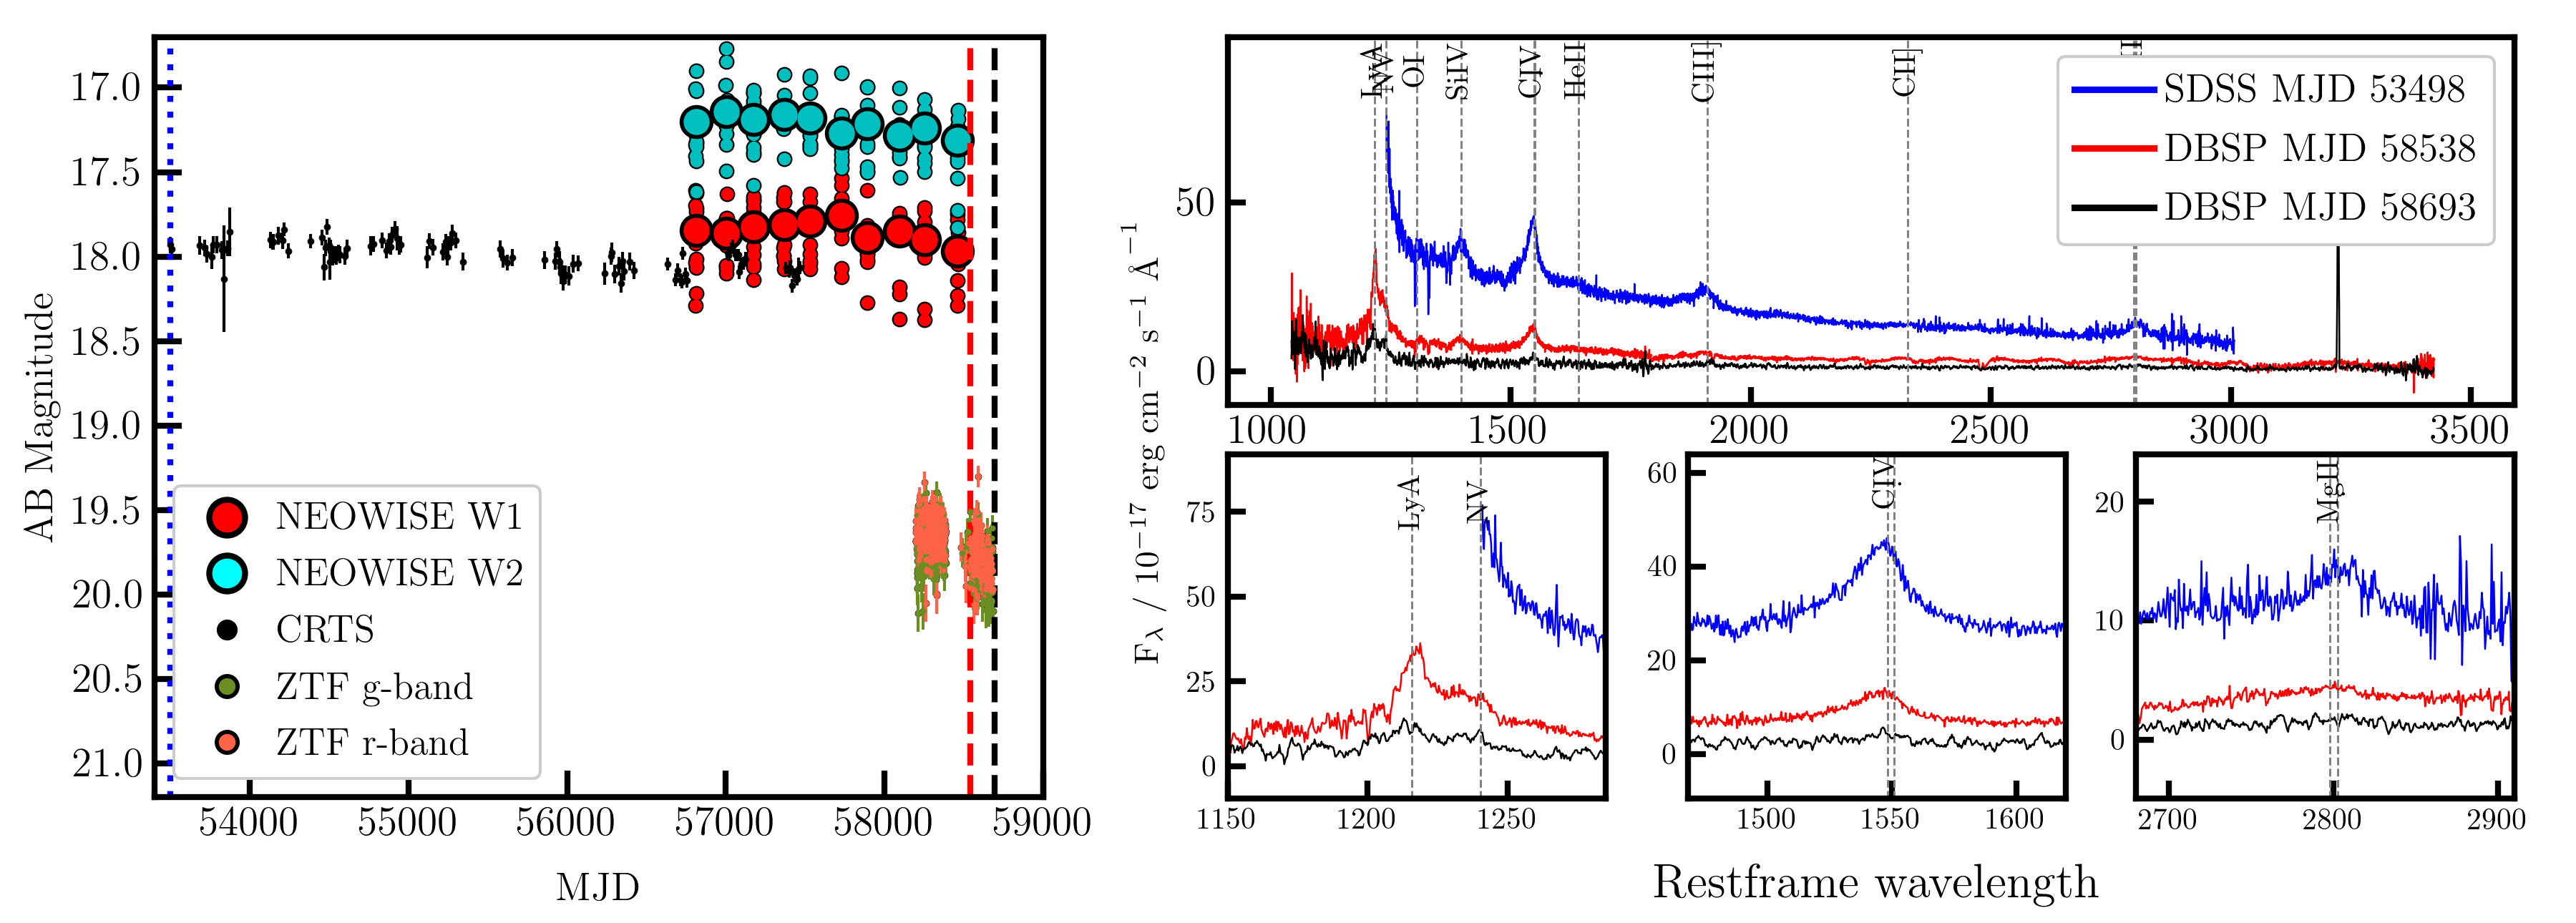
\includegraphics[width=16.7cm, trim=0.3cm 0.05cm 0.45cm 0.1cm, clip]
  {figures/J1205+3422_landscape_20191024.png}
  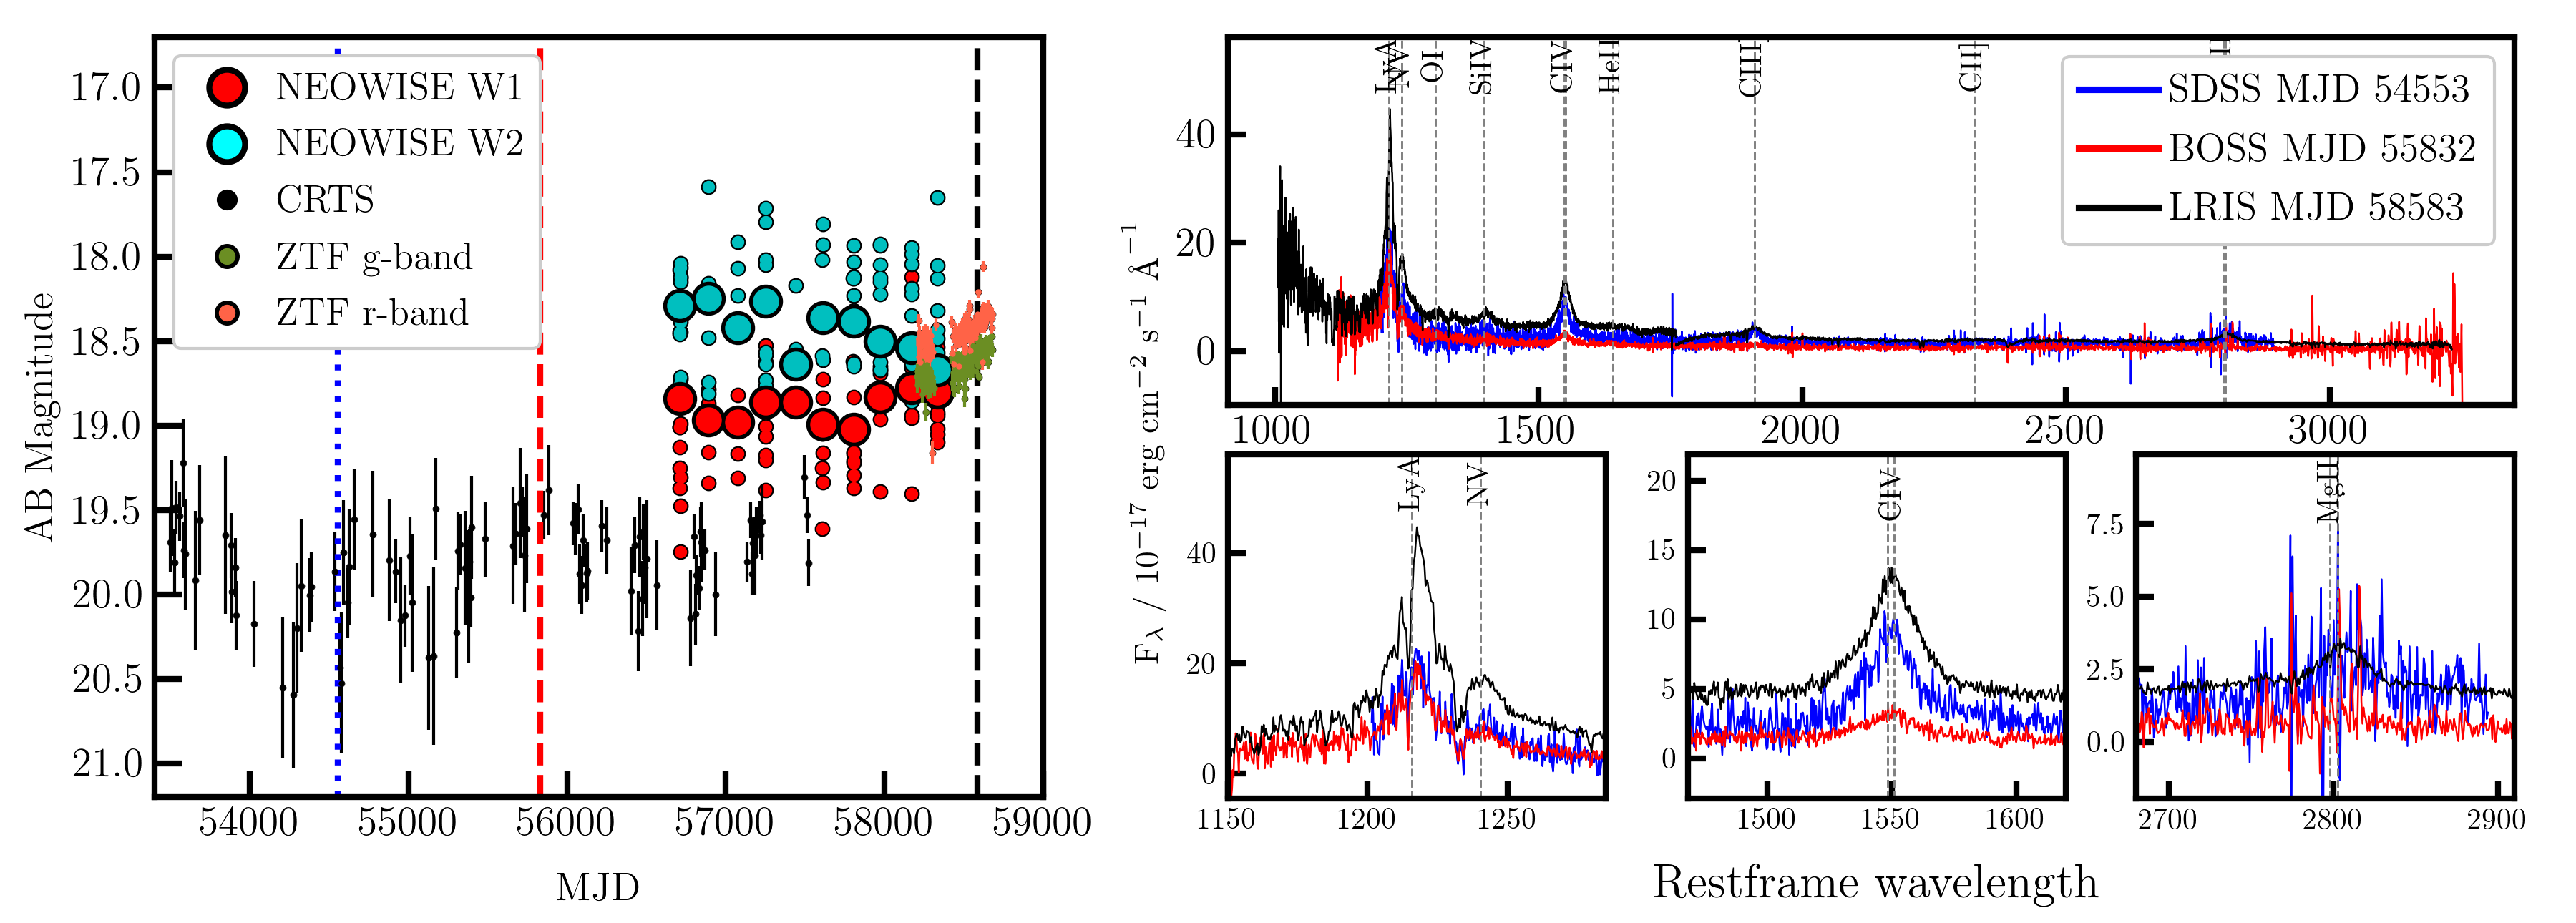
\includegraphics[width=16.7cm, trim=0.3cm 0.05cm 0.40cm 0.1cm, clip]
  {figures/J1638+2827_landscape_20191024.png}
  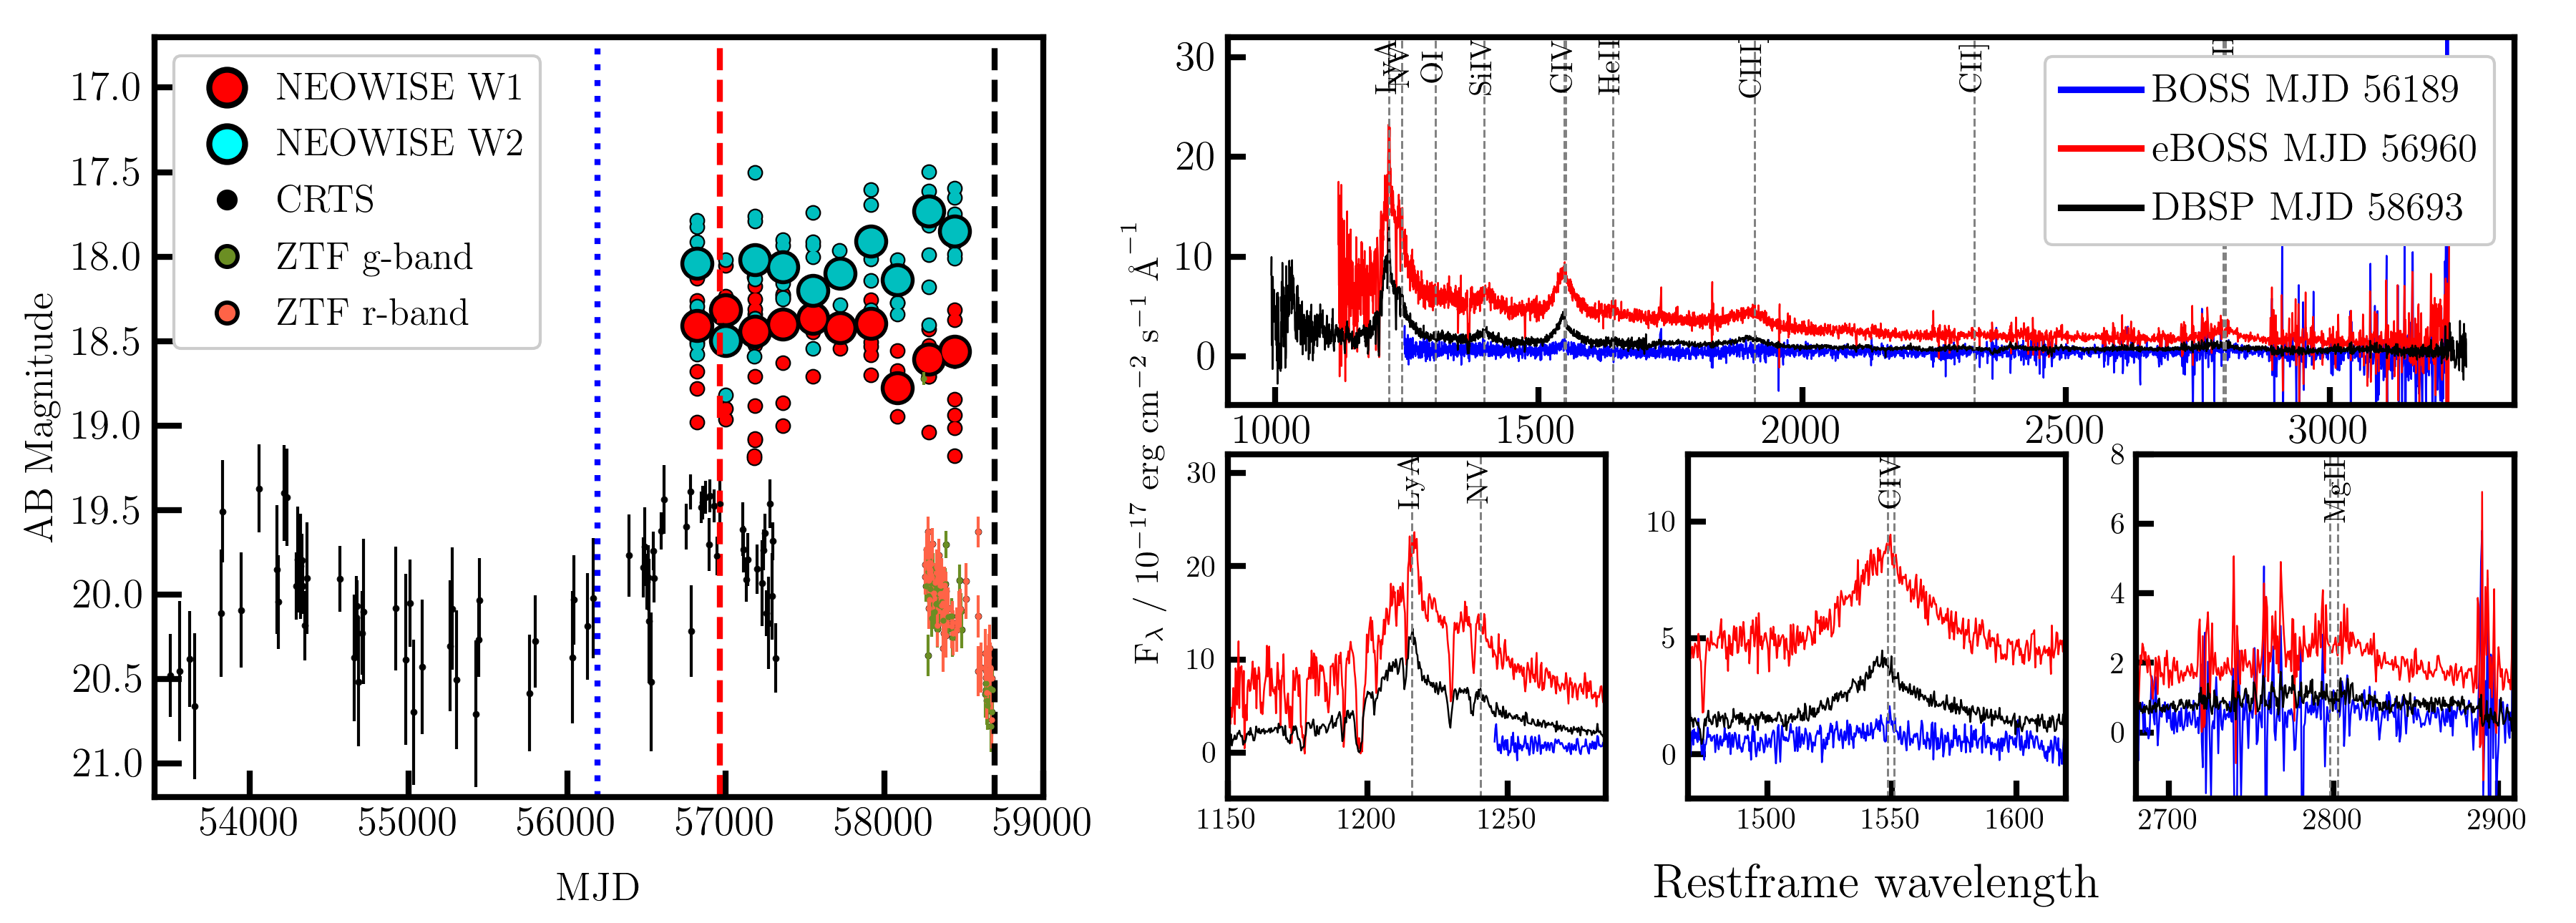
\includegraphics[width=16.7cm, trim=0.3cm 0.0cm  0.35cm 0.1cm, clip]
  {figures/J2228+2201_landscape_20191024.png}
  \vspace{-12pt}
  \caption[]{The threes high-$z$ CLQ quasars; 
    SDSS J1205+3422 (top), 
    SDSS J1638+2827 (middle), 
    SDSS J2228+2201 (bottom). 
The light curve data is present in the panels on the left hand side, with the 
spectral epoch observational timings given by the vertical lines. 
The spectra are on the right hand side, with zoom-in's on the Ly$\alpha$-\nv 
complex, the \civ\ line and the \mgii line. 
  }
  \label{fig:civ_clqs}
\end{figure*}
\subsection{Spectra}
An overview of our spectroscopic observations is given in
Table~\ref{tab:obs_notes}.  The spectra are from the SDSS
\citep{Stoughton2002, DR7, Schneider2010}, the SDSS-III Baryon
Oscillation Spectroscopic Survey \citep[BOSS][]{Eisenstein2011,
Dawson2013, Smee2013, Alam2015, Paris2017} and the SDSS-IV Extended
Baryon Oscillation Spectroscopic Survey \citep[eBOSS; ][]{Dawson2016,
Abolfathi2018, Paris2018}.  These quasars were targetted via a range
of techniques and algorithms \citep[see ][]{Richards2002, Ross2012,
Myers2015}. The SDSS, BOSS and eBOSS data are supplemented by
spectra from the Low Resolution Imaging Spectrometer (LRIS) on the 10m
Keck {\sc I} telescope \citep{Oke1995}.  and the Double Spectrograph
(DBSP) instrument on the Palomar {\it Hale} 5m telescope.


\subsection{Emission Line and Power-law slope measurements}
We use the measured quasar emission line properties from several catalogues: 
\citet{Shen2011}, \citet{Hamann2017}, \citet{Kozlowski2017} and
\citet{Calderone2017}.

\citet{Shen2011} present a compilation of properties of the 105,783
quasars in the SDSS Data Release 7 (DR7) quasar catalog \citep[DR7Q;
][]{Schneider2007}. \citet{Shen2011} report non-zero \civ\ FWHM and
EWs for approximately half (51,501) of the full DR7Q, and non-zero
\mgii FWHM and EWs for 80\% (84,183) of the DR7Q quasars).
%%
Measured line values using the methods and catalogue from
\citet{Shen2011}.  $M_{\rm I}(z=2)$ is the Absolute $i$-band magnitude
$K$-corrected to $z = 2$; Bolometric luminosity computed from the
monochromatic luminosity at 1350\AA\ using the spectral fits and
bolometric corrections (BC = 3.81) in \citet{Richards2006b}; Line
luminosity, FWHM, rest-frame equivalent width, and their errors for
the whole \civ\ profile.  Power-law slope $\alpha_{\lambda}$ for the
continuum fit for \civ; Virial BH masses using calibrations of
\citet{VestergaardPeterson2006}.  Eddington ratio computed using the
virial BH mass.


\citet{Calderone2017} present the Quasar Spectral Fitting (QSFIT)
software package which among other quantities provides luminosity
estimates as well as width, velocity offset and equivalent width of 20
emission lines, including \civ, \ciii and \mgii.  We attempt to process and fit
all nine spectra using the lastest version (v1.3.0) of the QSFIT
\href{https://qsfit.inaf.it/cat_1.30/onlinefit.php}{online calculator}
and setting $E(B-V)=0.00$.

\citet{Hamann2017} investigate in robust detail the UV continuum and
the \civ\ (and \nv $\lambda$1238, 1242 \AA\ ) emission lines for over
200,000 quasars in BOSS DR12Q \citep{Paris2017}.  The quasar redshift
are limited to the range $1.53 \leq z \leq 5.0$ so that \civ\ and the
adjacent continuum are covered by BOSS. These measurements provide
line profile information and flux ratios\footnote{This emission-line
catalog can be downloaded from
\href{https://datadryad.org/stash/dataset/doi:10.6086/D1H59V}{here}.}
\citet{Hamann2017} was focused on $z\geq2$ quasars and specifcally
their \civ properties in order to understand the high-$z$ ``Extremely
Red Quasar'' population \citet{Ross2015, Zakamska2016, Perrotta2019,
Zakamska2019}.  As such, these measurements can be taken as the `gold
standard' for \civ line measurement, though this is only for two out of
our nine spectra.

When using the \citet{Shen2011} catalogue, we report line luminosity,
FWHM, rest-frame equivalent width, and their errors for the whole
\mgii profile (this catalogue also quotes values for just the broad
\mgii component, but the differences for our objects is
negligible). The line luminosities in \citet{Calderone2017} are given
in units of $10^{42}$ erg s$^{-1}$, while the line luminosities in
\citet{Shen2011} are in units of $\log(L)$.  We do not report the
\citet{Shen2011} error on the line luminosity.

Power-law continuum slopes, $\alpha$, where $f_{\lambda} \propto
\lambda^{\alpha}$, are also reported in these catalogues and from
QSFit.  We quote the most appropriate value given the emission line
wavelength.

\subsection{Multi-wavelength properties}
Mid-infrared data (3.4 and 4.6$\mu$m) is available from the beginning of the
Wide-field Infrared Survey Explorer (WISE) mission \citep[2010
January; ][]{Wright2010} through the fifth-year of NEOWISE-R
operations \citep[2018 December; ][]{Mainzer2011}. The WISE scan
pattern leads to coverage of the full-sky approximately once every six
months (a ``sky pass''), but the satellite was placed in hibernation
in 2011 February and then reactivated in 2013 October. Hence, our
light curves have a cadence of 6 months with a 32 month sampling gap.
%Radio ??



%%%%%%%%%%%%%%%%%%%%%%%%%%%%%%%%%%%%%%%%%%%%%%%%%%%%%%%%%%%%%%%%%%%%%%%%%%%%%
%%%%%%%%%%%%%%%%%%%%%%%%%%%%%%%%%%%%%%%%%%%%%%%%%%%%%%%%%%%%%%%%%%%%%%%%%%%%%
%%
%%   SECTION 3   SECTION 3   SECTION 3   SECTION 3   SECTION 3   SECTION 3  
%%   SECTION 3   SECTION 3   SECTION 3   SECTION 3   SECTION 3   SECTION 3  
%%   SECTION 3   SECTION 3   SECTION 3   SECTION 3   SECTION 3   SECTION 3  
%%
%%%%%%%%%%%%%%%%%%%%%%%%%%%%%%%%%%%%%%%%%%%%%%%%%%%%%%%%%%%%%%%%%%%%%%%%%%%%%
%%%%%%%%%%%%%%%%%%%%%%%%%%%%%%%%%%%%%%%%%%%%%%%%%%%%%%%%%%%%%%%%%%%%%%%%%%%%%
\section{Results}
\subsection{Overall Spectral Evolution}
Figure~\ref{fig:civ_clqs} presents the optical and infrared light
curves for three high-$z$ CLQ quasars.  Figure~\ref{fig:civ_clqs} also
shows the spectra for each epoch, with the MJD of observation given by
the dashed vertical lines in the light curves.

For J1205+3422, our spectral observations cover 5195 days observed, 1691 days
in the rest-frame. For J1205+3422 is identified in SDSS as a bright
$g\approx18.0$, blue-sloped quasar with broad \siiv, \civ, \ciii and
\mgii observed in the initial spectrum (MJD 53498; 2005-May-08). \ciii
and \civ\ are seen to have large blueshifts of $\approx$2600$\pm$150
and $\approx$1150$\pm$100 km s$^{-1}$, respectively.  By the time the
2019 spectra were taken (MJD 58538, 2019-Feb-24 and MJD 58693
2019-Jul-29), however, the light curve has dropped by $\sim$1.5
magnitudes and the spectra are significantly less steep.  While \lya
and \nv are detectable in both the MJD 58538 and MJD 58693 DBSP
spectra, \civ\ has all but disappeared in the MJD 58693 spectrum.  The
broad \ciii emission has disappeared between the 2005 and 2019
spectra. {\it The changes in \civ\ and \ciii going from broad emission to
barely detectable have on the timescales of $\approx$50 days in the rest-frame.} 

For J1638+2827, our spectral observations cover 4030 days observed, 1265 days
in the rest-frame. Here, in the initial epoch spectrum, \civ\ is broad
and bright, as is \ciii. However, just over 400 days in the rest-frame
later, the broad \civ\ and \ciii BEL have to faded, the continuum
slope around 1400\AA\ has changed from $\approx$-1.48 to
$\approx$-2.25, but the \lya/\nv emission complex is very similar in
shape and line flux intensity. Around 870 days in the rest-frame after
the second spectral epoch, \lya, \nv, \civ, \ciii and \mgii are all
apparent and broad, with \mgii being seen for the first time at high
signal-to-noise. The light curve is consistent with this spectral
brightening, increasing from around $\sim$19.5-20.5th magnitude to
$\sim$18.5 in the optical band. An absorption feature between  \lya and \nv
is seen in all three spectral epochs. 

For J2228+2201, our spectral observations cover 2504 days observed,
778 days in the rest-frame. Over the course of 240 days in the rest-frame, \civ\ and \ciii both {\it emerge} as BELs and
the standard UV/blue continuum slope increases in flux.
Then, over the course of 538 days in the rest-frame, the broadline emission, while still
very present, reduces in line flux the UV/blue continuum diminishes,
though is still more luminous than the initial BOSS spectrum. 




\begin{figure}
  \centering
  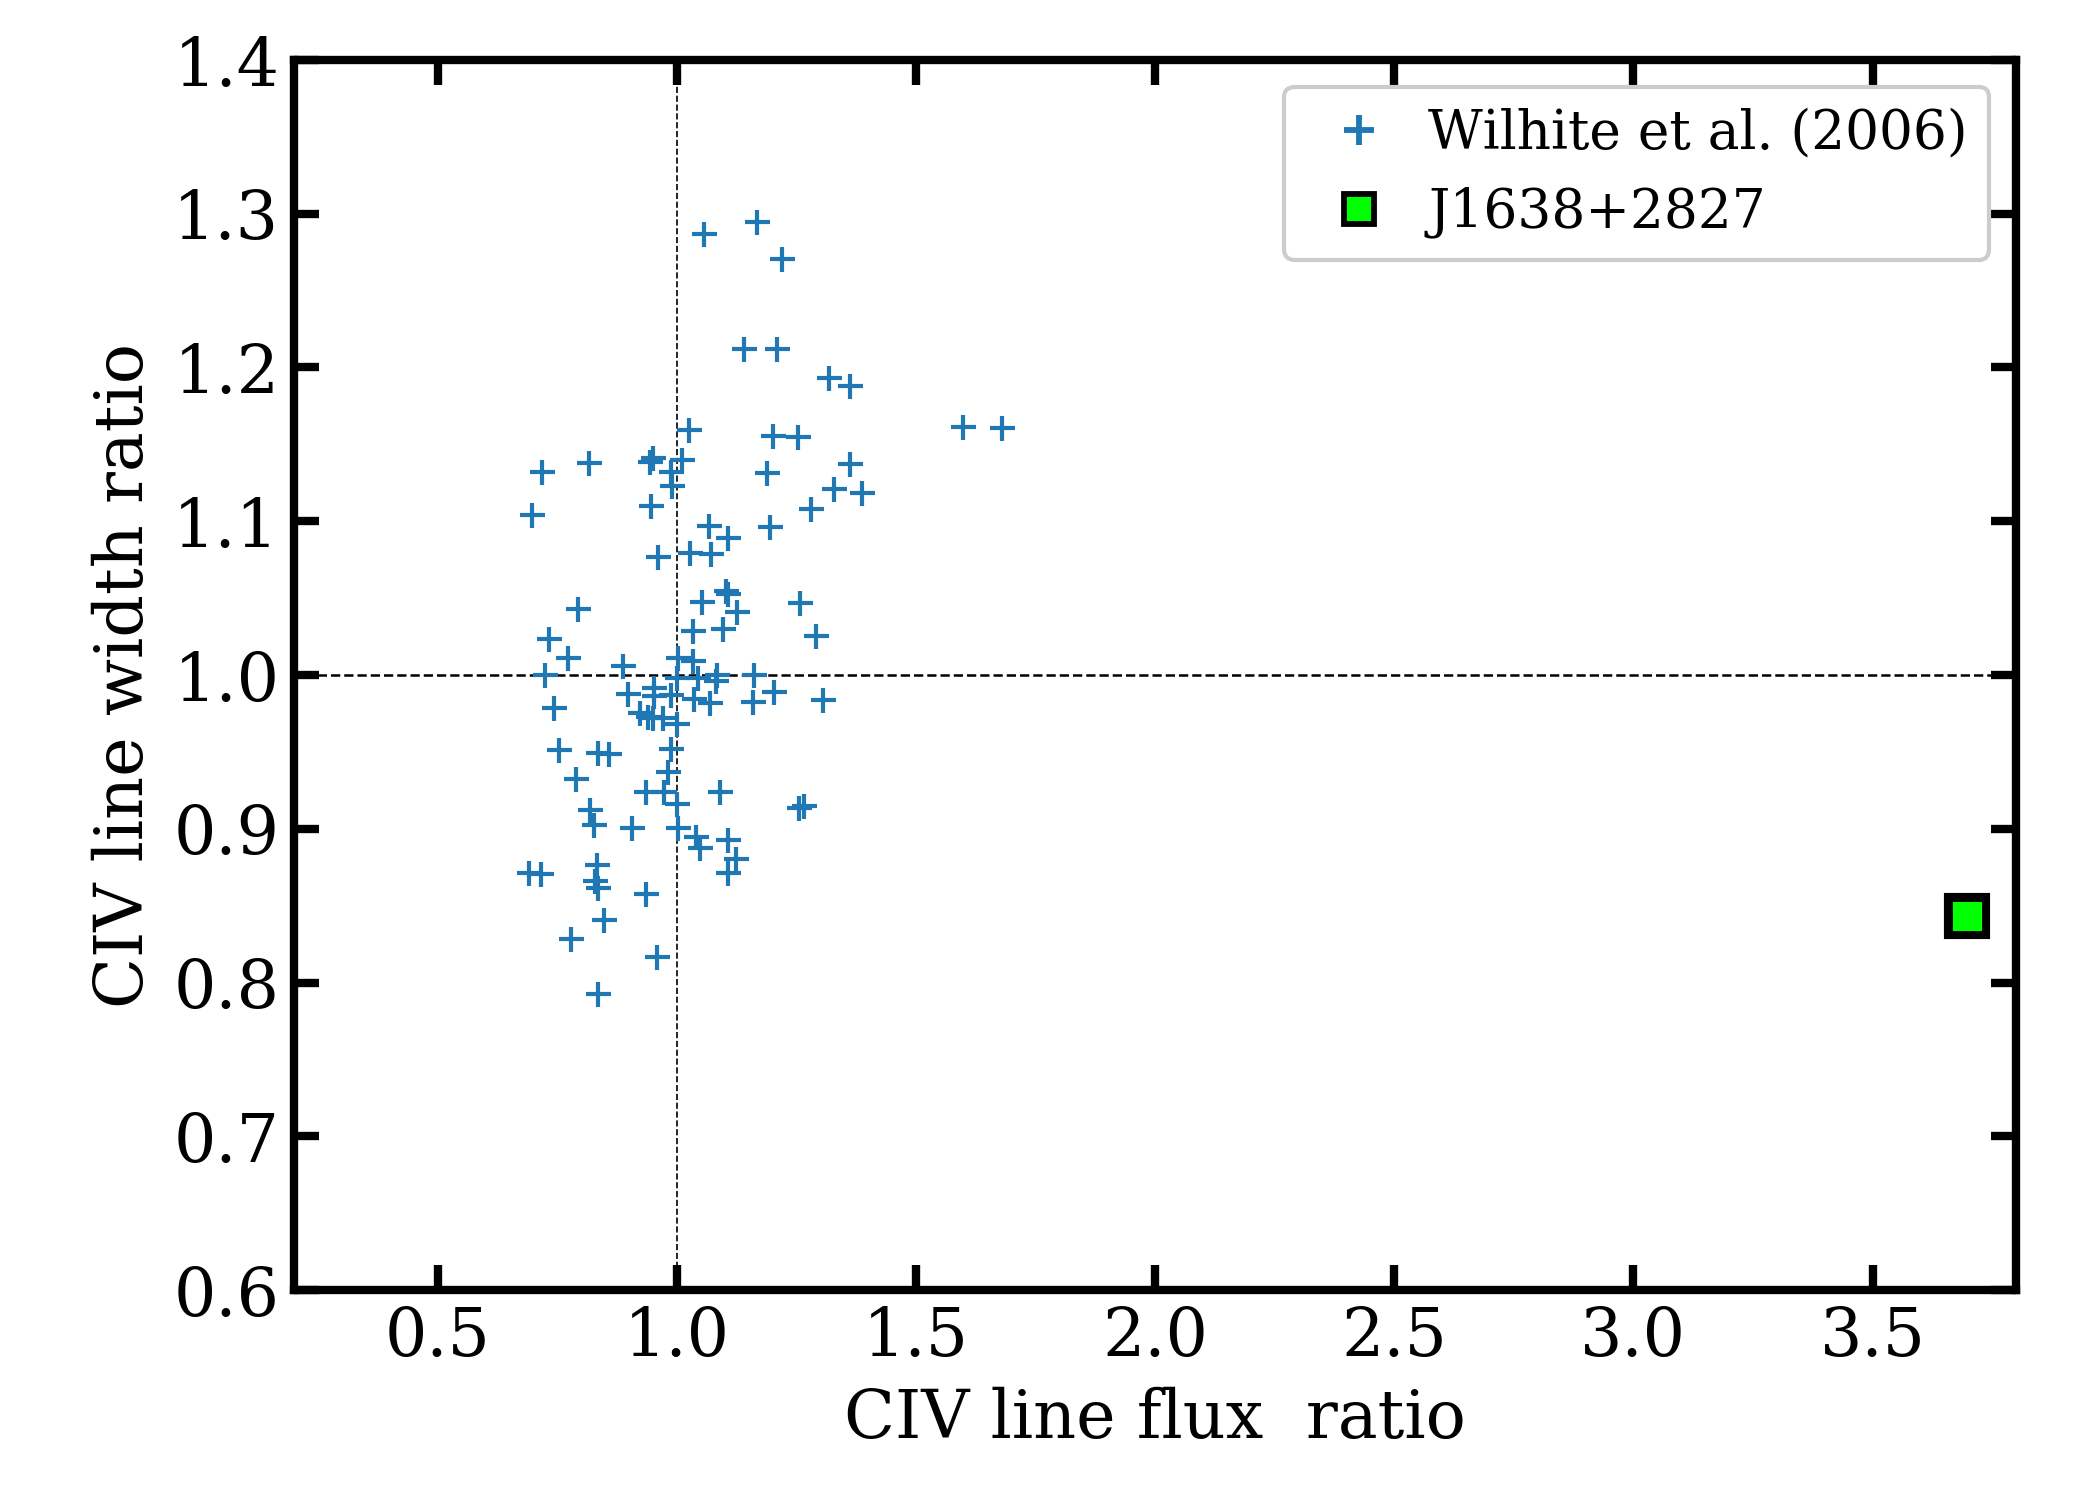
\includegraphics[width=8.7cm, trim=0.2cm 0.2cm 0.2cm 0.2cm, clip]
  {figures/Wilhite_2006_Fig2_redux_20190926.png}
   \vspace{-12pt}
  \caption[]{The Change in \civ\ line width vs. line flux change. 
We compare our object J1638+2827 with the sample 
from \citet{Wilhite2006} with a sample of 105 quasars observed at
multiple epochs by the SDSS. J1638+2827 is a substantial outlier 
in this parameter space.}
  \label{fig:Wilhite2006_comparison}
\end{figure}
\subsection{Overall Spectral Evolution}
Emission line measurements from the catalogues of  \citet{Shen2011}.
\citet{Hamann2017}, \citet{Kozlowski2017} or the QSFit routine of \citet{Calderone2017}
are presented in Table~\ref{tab:LineMeasurement}.
%%
From Figure~\ref{fig:Wilhite2006_comparison} there appears to be a
strong correlation between the change in the line flux and the change
in the line width.  Figure~\ref{fig:Wilhite2006_comparison} shows the
epoch-to-epoch flux ratio versus the ratio of line widths.

The Balmer series in hydrogen is due to the recombination cascade
between different principal quantum numbers $n$, and
the $n=2$ level \citep[e.g., ][]{Seaton1959a, Seaton1959b}. 
%(and assuming an equilibrium distribution between the angular momentum levels $l$ corresponding to a given $n$).
%%
Lower redshift $z<0.9$ CLQs have traditionally been identified via large changes in the
H$\beta$ emission line. H$\beta$ emission is associated with a 2.55 eV energy difference. 
Thus we can place the high-$z$, HIL \civ\ in context of Balmer H$\beta$ CLQs at lower-$z$. 
%%
\civ\ is one of the strongest collisionally excited lines in quasar
spectra \citet[e.g.][]{HamannFerland1999}.  The line is most prominent
at n H $\approx$10$10$ cm$-3$ and log $U$$\approx$-1.5, which are the
canonical BELR parameters deduced over from early analysis of the
\civ\ emission \citep{Davidson_Netzer1979}.  A dimensionless
ionization parameter $U\equiv \Phi(H) / c n_{H}$, where $c$ is the
speed of light and $n_{H}$ is the total hydrogen density (H$^{0}$ +
H$^{+}$).


\begin{table*}
  \centering
  % \begin{tabular}{lll  cccc r }
  \begin{tabu}{l ll  lccc c r }
    \hline 
    \hline 
    Object                               &   MJD      & line      & Line  Lumin.       &  FWHM                       &  $V_{\rm off}$         & E.W.                          & $\alpha_{\lambda}$   &   Catalogue \\                                   
    \hline                                     
    \rowfont{\color{blue}}       & 53498    & \civ      &  511$\pm$13    &   9593$\pm$287        &  1172$\pm$74      & 15.9$\pm$0.4      & $-1.64\pm0.01$      &     QSFit \\
    \rowfont{\color{blue}}       & 53498    & \civ      &  787                   &   5230$\pm$219        &  1118$\pm$133    & 30.1$\pm$1.21    & $-1.47\pm0.08$     &     Shen2011 \\
    \rowfont{\color{blue}}       & 53498    & \civ      &   403                  &   5119$^{(a)}$             &    ---                     &  ---                        &  ---                        &     DR12 SAS   \\
                                             & 53498     & \ciii      &  441$\pm$10   & 14959$\pm352^{(b)}$ &  2616$\pm$147    & 25.10$\pm$0.59    & $-1.65\pm0.01$     &     QSFit   \\
                                             & 53498    & \ciii       &   144                 &   5119$^{(a)}$             &  ---                       &   ---                       &  ---                         &       DR12 SAS  \\
  \rowfont{\color{teal}}         & 53498     & \mgii     &  327$\pm$20   &   4907$\pm$387       &  $-274\pm419$     & 26.66$\pm$1.65    &   $-1.65\pm0.01$    &  $^{(d)}$QSFit  \\
  \rowfont{\color{teal}}         & 53498     & \mgii     &  284                  &   4730$\pm$314       &  $-179\pm188$     & 32$\pm$3.88         &  $-1.87\pm0.06$    &       Shen2011 \\
 \multirow{2}{*}{{\bf J1205+3422}}  
                &     \textcolor{teal}{53948}     & \textcolor{teal}{\mgii}   & \textcolor{teal}{130} & \textcolor{teal}{5119$^{(a)}$}   &  \textcolor{teal}{---}   & \textcolor{teal}{---}        & \textcolor{teal}{---}    & \textcolor{teal}{DR12 SAS}    \\
                                 \cdashline{2-9}
                                            & 58538     & \lya      & 1393$\pm$11   & $>$15000            &  $-796\pm57$          &  ---                        &  ---                       &   QSFit (NPR) \\
                                            & 58538     & \lya      & 952$\pm$1.1    & 12242$\pm$15    &  $-1679\pm6$          &  165$\pm$0.2        &  ---                       &   QSFit (MJG) \\
   \rowfont{\color{blue}}       & 58538     & \civ      & 1037$\pm$5    & $>$15000             &  983$\pm$40            &  ---                        &  ---                       &   QSFit (NPR)   \\
    \rowfont{\color{blue}}      & 58538     & \civ      &       0$\pm$-    & 14995$\pm$0       & $>$3000$\pm$         &  ---                       &  ---                       &   QSFit (MJG)    \\  
                                            & 58538      & \ciii     &  677$\pm$4     & $>$15000             & $>$3000                    &  5770$\pm$34       &  ---                       &  QSFit (NPR) \\  
                                            & 58538      & \ciii     &  167$\pm$0.9  & $>$15000            &  2734$\pm$46            &     45$\pm$0.2       &  ---                       &  QSFit (MJG)  \\
    \rowfont{\color{teal}}      & 58538     & \mgii    &  755$\pm$4     & $>$15000            & 350$\pm$39               &  7571$\pm$37       &  ---                       &   QSFit (NPR) \\
    \rowfont{\color{teal}}      & 58538     & \mgii    &  216$\pm$1.4  & 13940$\pm$94    & $-465.2\pm38$         &  88$\pm$0.6	    &  ---                       &   QSFit (MJG) \\
                                          \cdashline{2-9}
                                           & 58693     & \lya     &  290$\pm$3       & 8803$\pm$52     &  $-1096\pm35$        &  ---                           & $<$-3                   &   QSFit (NPR)\\
                                           & 58693     & \lya     &  271$\pm$0.9    & 9637$\pm$52     &  $-447\pm13$          &  85.1$\pm$0.3          & ---                        &   QSFit (MJG) \\ 
    \rowfont{\color{blue}}    & 58693     & \civ      &   68$\pm$0.9    & 3743$\pm$26     &   591$\pm$17           &   ---                           & $<$-3                   &  QSFit (NPR)\\  
    \rowfont{\color{blue}}    & 58693     & \civ      &   52$\pm$0.9    & 5046$\pm$26     &   1053$\pm$17         &   24.0$\pm$0.2          & ---                        &  QSFit (MJG)  \\  
                                           & 58693     & \ciii     &   19$\pm$0.4    & 5625$\pm$          &   $>$3000                 &  988$\pm$20             & $<$-3                   &  QSFit (NPR) \\  
                                           & 58693     & \ciii     &   59$\pm$0.9    & 10751$\pm$        &  1097$\pm$77         &   36$\pm$0.6             & ---                        &  QSFit (MJG)  \\  
   \rowfont{\color{teal}}      & 58693     & \mgii    &  19$\pm$0.4    & 1530$\pm$22      &  $>$3000                  &    499$\pm$9             &$<$-3                    &  QSFit (NPR)  \\
   \rowfont{\color{teal}}      & 58693     & \mgii    &  69$\pm$1.5    & 14983$\pm$346   &  $-190\pm134$       &    72$\pm$1.6           & ---                        &  QSFit (MJG)  \\  
\hline
                                                & 54553     & \lya      & 188                 &  3207                     &    ---                        &   ---                         & ---                    &   DR12 SAS  \\
   \rowfont{\color{blue}}          & 54553     & \civ      & 257$\pm$13   &  4550$\pm$371     &   55$\pm$450         &   31.8$\pm$1.5     &                                &  $^{(d)}$QSFit  \\
   \rowfont{\color{blue}}          & 54553     & \civ      & 281                  &    4181$\pm$736   &    680$\pm$133       & 100.5$\pm$12  & $-0.14\pm0.68$    &  Shen2011   \\
   \rowfont{\color{blue}}          & 54553     & \civ      & 170                  &   4537$^{(a)}$        &    ---                       &   ---                         & ---                         &  DR12 SAS  \\
                                                & 54553     & \ciii     &  130$\pm$10   &  3852$\pm$402    &  $-236\pm565$       &  36.7$\pm$2.8          &  $-1.47\pm0.20$    &  $^{(d)}$QSFit  \\
                                                & 54553     & \ciii     &  61                    &  4537$^{(a)}$          &  ---                         &  ---                           & ---                         &  DR12 SAS \\
    \rowfont{\color{teal}}          & 54553      & \mgii  &  139                  &  4757$\pm$2224   &  $-944\pm568$        &   119$\pm$40          &  $-1.49\pm0.54$    &  Shen2011   \\
    \rowfont{\color{teal}}          & 54553      & \mgii  &  69                    &  4537$^{(a)}$           &    ---                        &  ---                          & ---                          &  DR12 SAS  \\
                                                \cdashline{2-9}
                                                & 55832     & \lya     & 288$\pm$11    &  4444$\pm$243       &  -463$\pm$68         &  103.69$\pm$3.99   &                               &   QSFit  \\
                                                & 55832     & \lya     & 234                  &  4165.6$^{(a)}$         &    ---                       &   ---                         & ---                         &   DR12 SAS  \\ 
\multirow{2}{*}{\bf {J1638+2827}}
 & \textcolor{blue}{55832} & \textcolor{blue}{\civ}    & \textcolor{blue}{63$\pm$3}  &   \textcolor{blue}{6052$\pm$250}  &  \textcolor{blue}{-117$\pm$103}  &  \textcolor{blue}{43.2$\pm$1.7}  &  \textcolor{blue}{-2.25$\pm$0.05} & QSFit    \\
    \rowfont{\color{blue}}           &  55832   &  \civ     &  ---               &    5210$\pm$226     &    ---                       &   42.8$\pm$2.0         & $-3.35$                 &     Ham17  \\
    \rowfont{\color{blue}}           &  55832   &  \civ     &  46                 &    5385$^{(a)}$           &    ---                       &   ---                         & ---                         & DR12 SAS \\
                                                 & 55832     & \ciii     & 15$\pm$5     &  11421$\pm$3654   &   $>$3000                &   14.8$\pm$4.5         &  $-2.25\pm0.05$   &        QSFit \\
                                                 &  55832    &  \ciii    &  11                 &     5385$^{(a)}$         &  ---                          &    ---                         &  ---                       &   DR12 SAS \\  
    \rowfont{\color{teal}}           &  55832     & \mgii   &  13                &     5385$^{(a)}$         &  ---                           &   ---                          &  ---                       &   DR12 SAS\\  
                                               \cdashline{2-9}
                                               & 58583       & \lya    &  1086$\pm$14  & $>$15000     	&   $-1047\pm88$        &  500$\pm$6   	  & $-0.443\pm0.01$   & QSFit (NPR)\\ 
                                               & 58583       & \lya    &  785$\pm$1      & 4956$\pm$4    	&   $-641\pm2$            &   90$\pm$0.1   	  &  ---                          & QSFit (MJG) \\
   \rowfont{\color{blue}}         & 58583      & \civ      &  659$\pm$5     & $>$15000                &  $-493\pm56$          &   333$\pm$3           & $-0.43\pm0.01$     &   QSFit (NPR)  \\
   \rowfont{\color{blue}}         & 58583      & \civ      &  311$\pm$1     & 5739$\pm$14	 &  $-167\pm6$             &   58$\pm$0.1          & ---                          &   QSFit (MJG)  \\  
                                               & 58583      & \ciii      &  239$\pm$4    &  $>$15000               &  1514$\pm$127        &  124$\pm$2            & $-0.43\pm0.01$     &   QSFit (NPR) \\   
                                               & 58583      & \ciii      &  52$\pm$0.8   &  3917.4	68.837      &  1514$\pm$127        &  124$\pm$2             & ---                          &   QSFit (MJG) \\   
   \rowfont{\color{teal}}           & 58583      & \mgii   &  129$\pm$3    &  10957$\pm$307    &  138$\pm$128          &   78$\pm$2              & $-0.43\pm0.01$     &   QSFit (NPR) \\
   \rowfont{\color{teal}}           & 58583      & \mgii   &  157$\pm$2    &  10565$\pm$129    &  $-450\pm52$          &   92$\pm$1              & ---                          &   QSFit (MJG) \\  
\hline
    \rowfont{\color{blue}}         &  56189     & \civ    &   ---                 &   2994$\pm$620       &     ---                       &   42.2$\pm$5.6      & -1.59                      &    Ham17  \\
    \rowfont{\color{blue}}         &  56189     & \civ    &   19                  &    5218$^{(a)}$            &    ---                       &   ---                       &  ---                        &   DR12 SAS  \\
                                               &  56189      &  \ciii   &  34$\pm$6       &  13748$\pm$2869    &   1851$\pm$1140    &  63$\pm$12          &  $-0.46\pm0.21$    &   QSFit  \\
                                               &  56189      & \ciii    &  7                     &     5218$^{(a)}$          &  ---                         &     ---                     & ---                         &   DR12 SAS \\  
    \rowfont{\color{teal}}          & 56189      & \mgii  &  25$\pm$6       &   7253$\pm$1712     &   $-931\pm708$      &  51$\pm$10.95      &  $-0.46\pm0.21$   &   QSFit   \\
    \rowfont{\color{teal}}         &  56189      &  \mgii &  13                   &     5218$^{(a)}$          &  ---                         &   ---                        &  ---                       &   DR12 SAS \\  
                                                  \cdashline{2-9}
                                              & 56960         & \lya    & 121$\pm$38     & 3580$\pm$673       &     -16$\pm$171     &  13.52 $\pm$4.21    & ---                        &   QSFit   \\  
\multirow{2}{*}{{\bf J2228+2201}}
           & \textcolor{blue}{56960} & \textcolor{blue}{\civ}  & \textcolor{blue}{229$\pm$4}      &  \textcolor{blue}{8911$\pm$169}   &   \textcolor{blue}{92$\pm$68}  &   \textcolor{blue}{46.8$\pm$0.9}    & ---    & \textcolor{blue}{QSFit}     \\   
                                               & 56960    & \ciii      & 185$\pm$5        &        -                      &  2701$\pm$225      &   47.75$\pm$1.29     & ---                      &   QSFit    \\  
   \rowfont{\color{teal}}           & 56960    & \mgii   &   99$\pm$4        &  7312.6$\pm$340   &   188$\pm$137      &   50.75$\pm$2.21     & ---                      &   QSFit   \\
                                               \cdashline{2-9}
                                               & 58693     & \lya      &  228$\pm$3       & 4279$\pm$32       &   $-1000\pm29$     &  91976$\pm$1311  &  ---                       &  QSFit (NPR)\\ 
                                               & 58693     & \lya      &  447$\pm$5       & 8133$\pm$93       &   613$\pm$130       &        56$\pm$0.6     &  ---                    	 &   QSFit (MJG) \\
     \rowfont{\color{blue}}        & 58693     & \civ      &  327$\pm$1      &  $>$15000             &   $-453\pm34$       &  20298$\pm$106    & ---                        &  QSFit (NPR)\\  
     \rowfont{\color{blue}}        & 58693     & \civ      &  41$\pm$1        &  4914$\pm>$65    &   160$\pm$27         &   25$\pm$0.3          & ---                         & QSFit (MJG)  \\  
                                               & 58693     & \ciii      & 269$\pm$1.5    &  $>$15000             &  2302$\pm$42.6     &   3776$\pm$21      & ---                          &  QSFit (NPR) \\
                                               & 58693     & \ciii      & 107$\pm$1.2    &  $>$15000             &  2422$\pm$67        &   ---                       & ---                          &  QSFit (MJG)   \\  
     \rowfont{\color{teal}}        & 58693     & \mgii    & 177$\pm$1.1    &  $>$15000             &  1000$\pm$2617    &   16$\pm$36         & ---                           &   QSFit (NPR) \\
     \rowfont{\color{teal}}        & 58693     & \mgii    &  89$\pm$1.4     &  $>$15000             &  $>$1000                &   1230$\pm$1.9    & ---                            &   QSFit (MJG) \\  
\hline
\hline
     %    \end{tabular}
    \end{tabu}
    \caption{Line Measurement information for the nine epochs for the 3 quasars.
      Line Luminosity is in units of 10$^{42}$ erg s$^{-1}$; FWHM and $V_{\rm off}$ in km s$^{-1}$,
      where positive values of $V_{\rm off}$ means the line is blueshifted.
      Equivalent widths are \AA\.  
      Shen11 is \citet{Shen2011}. 
      Ham17 is \citet{Hamann2017}.
      DR12 SAS is the line measurement information from the SDSS DR12 
      Science Archive Server (SAS).
          $^{(a)}$Emission lines of a common ``width group'', in this case,
    \civ1549, \heii1640, \ciii1909 and \mgii2800 are constrained to have
    the same intrinsic velocity width in the SDSS spectral line fitting
    procedure \citep{Bolton2012}. 
      %$^{(a)}$ $\text{FWHM}=2\sqrt{2\sigma^2\ln 2}=\sigma\sqrt{8\ln 2}$.
      Positive values of Voff means the line is blueshifted.
%      $^{(b)}$Bit 3: FWHM value hits a limit in the fit
      Notes: QSFit does not fit the \mgii line for J1638+2827 MJD
      54553 or 55832. QSFit does not fit the \civ line for J2228+2201 MJD 56189.
      $^{(d)}$Emission line modelled with two components.
      The different colours of text are merely for readability.
    }
 \label{tab:LineMeasurement}
\end{table*}

%%
%% %% \eta_{\rm Edd} = log10((10**LBol)/((1.26e38)*(10**MBH)))
%%
%% Using    C IV

%% In [6]: log10((10**47.216)/((1.26e38)*(10**9.49)))                                                                                                                                             
%%Out[6]: -0.37437054511756207
%%
%%In [7]: log10((10**46.166)/((1.26e38)*(10**8.742)))                                                                                                                                            
%%Out[7]: -0.676370545117567
%%
%%In [8]: log10((10**46.721)/((1.26e38)*(10**9.1289)))                                                                                                                                           
%%Out[8]: -0.5082705451175662
%%
%%In [9]: log10((10**46.231)/((1.26e38)*(10**8.733)))                                                                                                                                            
%%Out[9]: -0.6023705451175618
\begin{table*}
  \begin{tabular}{l l  ll ll cc r}
    \hline
    \hline
\multirow{ 2}{*}{Object}  & \multirow{ 2}{*}{MJD} & \multirow{ 2}{*}{$M_i$} &  \multirow{ 2}{*}{$L_{\rm bol}$} & \multicolumn{2}{c}{$M_{\rm BH}$}     & \multicolumn{2}{c}{$\eta_{\rm Edd}$} &  Ref. \\
                                      &                                   &                                      &                                                 & \mgii                  & \civ                    &  \mgii           &  \civ                       &        \\
    \hline
                                     & 53498                         & -27.74                          & 47.216$\pm$0.004                 &  9.55$\pm$0.05  & 9.49$\pm$0.04   &     -0.434    & -0.374                   & Shen2011\\
 J1205+3422                & 58538                         &                                      &                                                 &                             &                             &                    &                               & \\
                                     & 58693                         &                                     &                                                  &                             &                             &                    &                               &   \\
    \hline 
                                    & 54553                          & -26.75                         & 46.166$\pm$0.04                    & 9.03$\pm$0.37    & 8.74$\pm$0.15  &  -0.964      & -0.677                      & Shen2011\\
 J1638+2827                & 55832                         &  -26.40                         & 46.721$\pm$0.073                 & 9.34                      &  9.13                    &  -0.717     & -0.509                          & Kol017\\
                                    & 58583                          &                                      &                                                &                               &                            &                   &                                      &  \\
    \hline 
                                   & 56189                          &  -25.46                         & 46.231$\pm$0.073                 &  9.45                     & 8.73                     &  -1.317   & -0.602                            & Kol017\\
J2228+2201               & 56960                          &                                       &                                                &                              &                               &                 &                                        & \\
                                  & 58693                          &                                       &                                               &                               &                                &                &                   &  \\
    \hline
    \hline
  \end{tabular}
  \caption{$\eta_{\rm Edd}$ is the base 10 logarithm of the Eddington ratio.
        Shen11 is \citet{Shen2011}. 
        Kol17 is \citet{Kozlowski2017}.
        Measured line values using the methods and catalogue from
\citet{Shen2011}.  $M_{\rm I}(z=2)$ is the Absolute $i$-band magnitude
$K$-corrected to $z = 2$; Bolometric luminosity computed from the
monochromatic luminosity at 1350\AA\ using the spectral fits and
bolometric corrections (BC = 3.81) in \citet{Richards2006b}; Line
luminosity, FWHM, rest-frame equivalent width, and their errors for
the whole \civ\ profile.  Power-law slope $\alpha_{\lambda}$ for the
continuum fit for \civ; Virial BH masses using calibrations of
\citet{VestergaardPeterson2006}.  Eddington ratio computed using the
virial BH mass.}
\label{tab:Eddington_ratios} 
\end{table*}


%%%%%%%%%%%%%%%%%%%%%%%%%%%%%%%%%%%%%%%%%%%%%%%%%%%%%%%%%%%%%%%%%%%%%%%%%%%%%
%%%%%%%%%%%%%%%%%%%%%%%%%%%%%%%%%%%%%%%%%%%%%%%%%%%%%%%%%%%%%%%%%%%%%%%%%%%%%
%%
%%   SECTION 4   SECTION 4   SECTION 4   SECTION 4   SECTION 4   SECTION 4  
%%   SECTION 4   SECTION 4   SECTION 4   SECTION 4   SECTION 4   SECTION 4  
%%   SECTION 4   SECTION 4   SECTION 4   SECTION 4   SECTION 4   SECTION 4  
%%
%%%%%%%%%%%%%%%%%%%%%%%%%%%%%%%%%%%%%%%%%%%%%%%%%%%%%%%%%%%%%%%%%%%%%%%%%%%%%
%%%%%%%%%%%%%%%%%%%%%%%%%%%%%%%%%%%%%%%%%%%%%%%%%%%%%%%%%%%%%%%%%%%%%%%%%%%%%
\begin{figure}
  \centering
  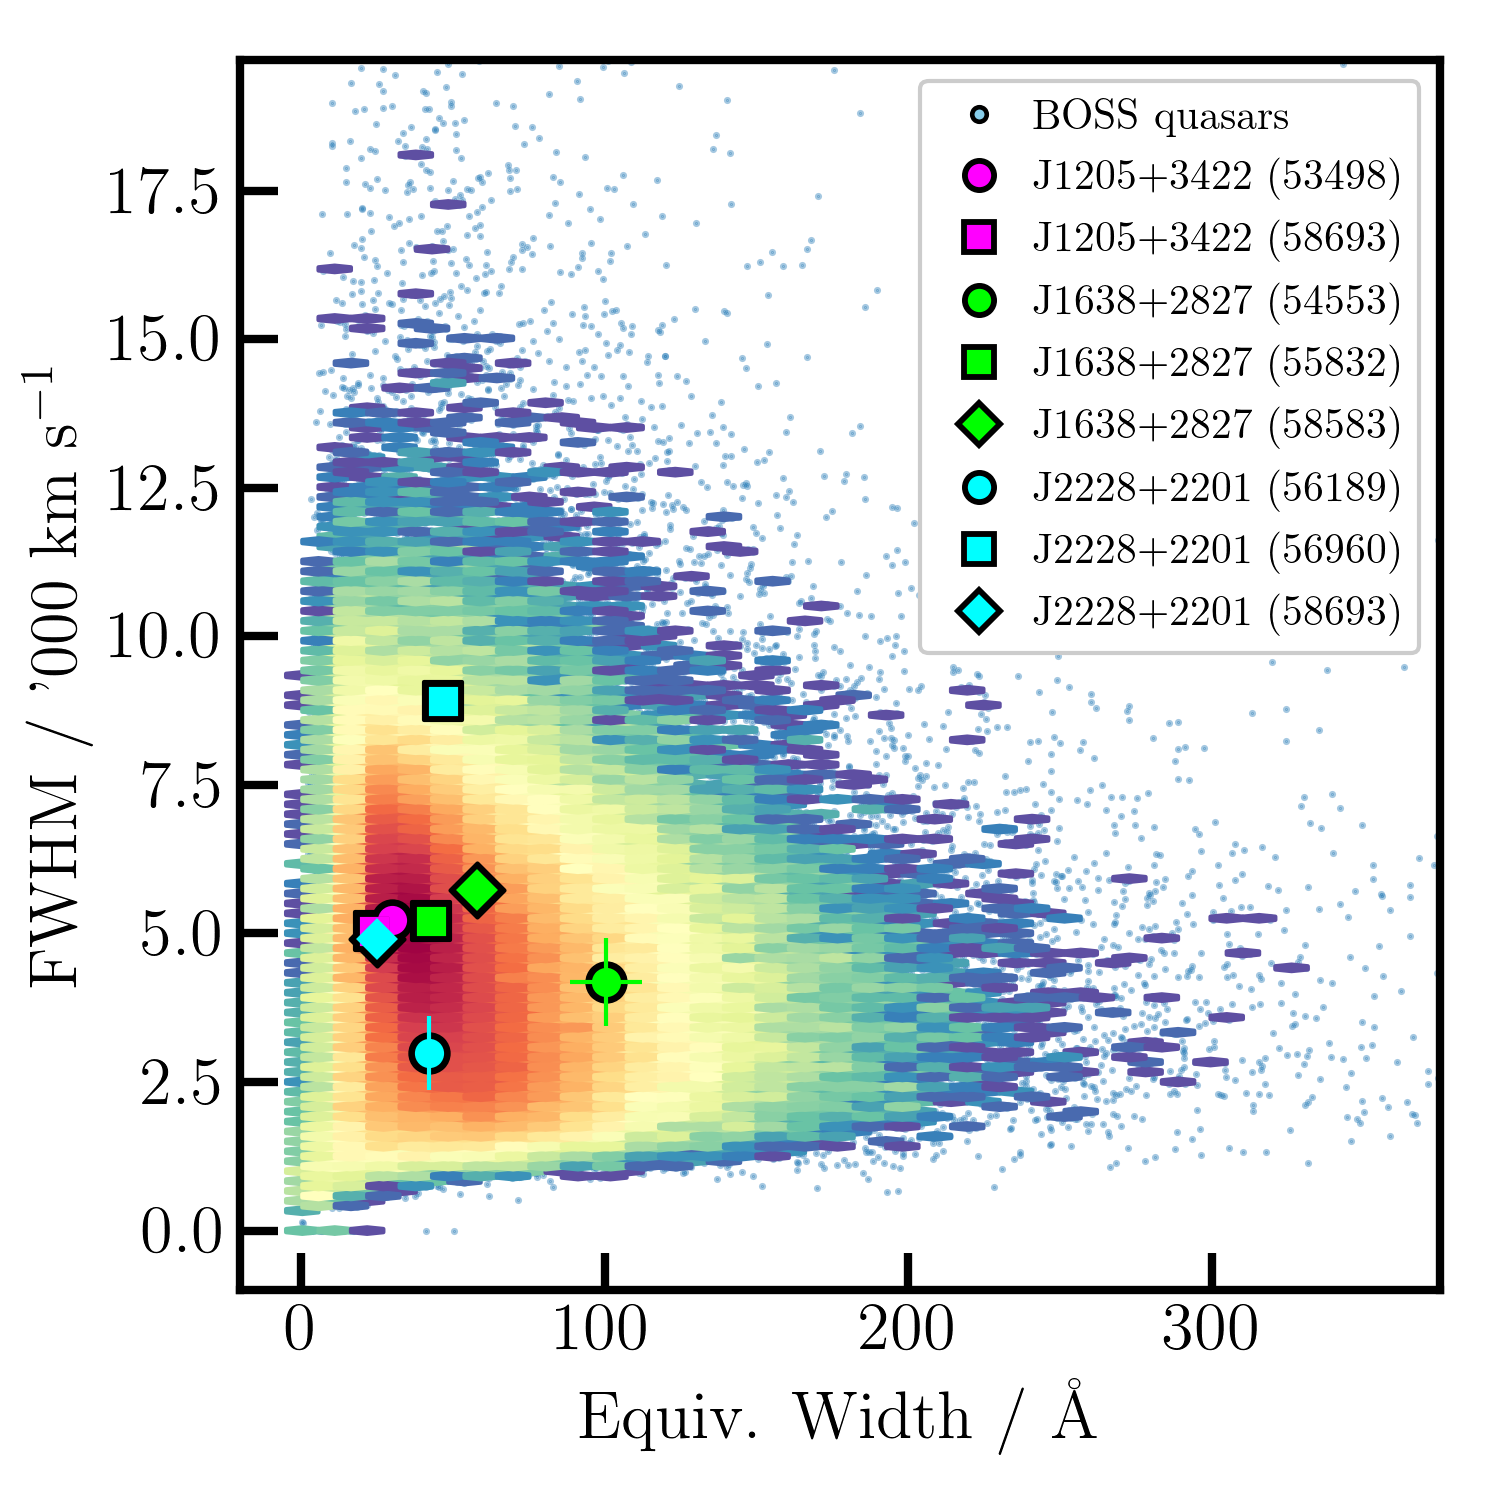
\includegraphics[width=8.7cm, trim=0.2cm 0.2cm 0.2cm 0.2cm, clip]
  {figures/CIV_CLQs_REWvsFWHM_20191029.png}
   \vspace{-12pt}
  \caption[]{The Rest Equivalent Width (REW) vs. Full Width Half Maximum (FWHM) 
of the \civ\ emission line in the BOSS DR12 quasar sample using the catalogue 
of \citet{Hamann2017}. Note the REW logarithmic scaling.}
  \label{fig:REWvsFWHM}
\end{figure}

%{\bf Our Eddington ratios \\
%Done 1\% \\
%Coatman, Hewett say \civ\ masses are okay.\\
%But what are these Eddington ratios? \\
%Low state BHs vs. High-mass BHs... \\
%Coatman et al?? Blue-shiftted \\ }
\section{Discussion}
\civ\ probes the photoionization environment produced by the innermost
disk, as indicated by RM time-delay measurements. In standard \citet{SS73}
thin disk models, large changes in the continuum flux are not
permitted over short timescales due to the relatively long viscous
time associated with such disks. Given the observed short timescale
continuum variations, it is not surprising that the \citet{SS73} disk may fail
on other fronts. The \civ\ variations observed in our sources... 
%DO/DO NOT (I can't tell!?! we have to determine this!) fit the Baldwin Effect relationship found by previous authors (cite em again).

%If they DO fit:
This indicates they may comfortably fit into the sample of CIV
variable QSOs explored by \citet{Dyer2019}, and similar to those
authors we suggest slim accretion disk models e.g., 
\citet[][]{Abramowicz1988} or inhomogeneous disk models
\citep[e.g.,][]{DexterAgol2011} may provide viable explanations for
our observations. I want to say a bit more here about the generic
probe of photoionization vs shielding and conditions in the BL region
but that will take more time.

%If they DO NOT fit:
This implies that the variable \civ\ in our sample arises through
different emission mechanisms than is usual for high-$z$ quasar...
%% --and I gotta think more/longer about what else to say here.


\subsection{The Baldwin Effect}
The variable properties of the rest-frame UV quasar emission lines
have been long studied, with the global (or ensemble) Baldwin Effect
(the anti-correlation between the EW of the emission line and the
underlying continuum luminosity of single-epoch observations of a
large number of AGN, first noted in \citet{Baldwin1977}.  More
recently, the intrinsic Baldwin effect, the same anti-correlation but
in an individual, variable AGN.  The variable properties of high-$z$
quasars, however, has been less well studied. Reasons for this include
more massive systems will tend to have longer timescales e.g. with
$R_{\rm Sch}= 2GM /c^{2}$ and $t_{\rm dyn} =\sqrt{ R^{3}/GM}$ means
$t_{\rm dyn} \sim 6 G^{3} M^{3} / GM c^{2} \sim 6G^{2} M^{2} / c^{2}
$.

The X-ray Baldwin Effect \citet[e.g., ][]{Iwasawa_Taniguchi1993}
\citet{Bachev2004} find a 10-fold decrease in EW C IV λ1549 with
Eddington ratio (decreasing from ~1 to ~0.01), while N V λ1240 shows
no change. These trends suggest a luminosity-independent ``Baldwin
effect'' in which the physical driver may be the Eddington ratio.
\citet{Ge2016} Broad emission lines is a prominent property of type I quasi-stellar objects (QSOs). 




\subsection{Eddington ratios and State Changes} 
The broad UV and optical lines in quasars are most sensitive to the
extreme ultraviolet (EUV) part of the spectral energy distribution
(SED), with \civ\ (and indeed \heii and \nv) being at the higher
energy end of the EUV distribution.

The soft X-ray excess – the excess of X-rays below 2 keV with respect
to the extrapo- lation of the hard X-ray spectral continuum model – is
a very common feature among type 1 active galactic nuclei (AGN). 
\citet{NodaDone2018} note that
The soft X-ray excess produces most of the ionizing photons, so its
dramatic drop leads to the disappearance of the broad-line region,
driving the ``changing-look'' phenomena.  major difference is that
radiation pressure should be much more important in AGNs, so that the
sound speed is much faster than expected from the gas temperature.
%%
This spectral hardening appears similar to the soft-to-hard state
transition in black hole binaries at $L / L_{\rm Edd} \sim 0.02$
(i.e. $\eta_{\rm Edd} \sim -1.7$, where the inner disc evaporates into
an advection dominated accretion flow, while the overall drop in
luminosity appears consistent with the hydrogen ionization disc
instability.  Crucially \citet{NodaDone2018} make the prediction that
all changing-look AGNs are similarly associated with the state
transition at $L / L_{\rm Edd} \sim$a few per cent.
%%
\citet{JiangYF2014, JiangYF2016, JiangYF2019}.
\citet{JiangYF2019arXiv} use global three dimensional radiation
magneto-hydrodynamic simulations to study the properties of inner
regions of accretion disks around a $5 \times 10^{8}$ M$_{\odot}$
black hole with mass accretion rates reaching 7\% and 20\% of the
Eddington value.

We investigate this reporting the Eddington ratios of the three
quasars in Table~\ref{tab:Eddington_ratios}.

\begin{figure}
  \centering
  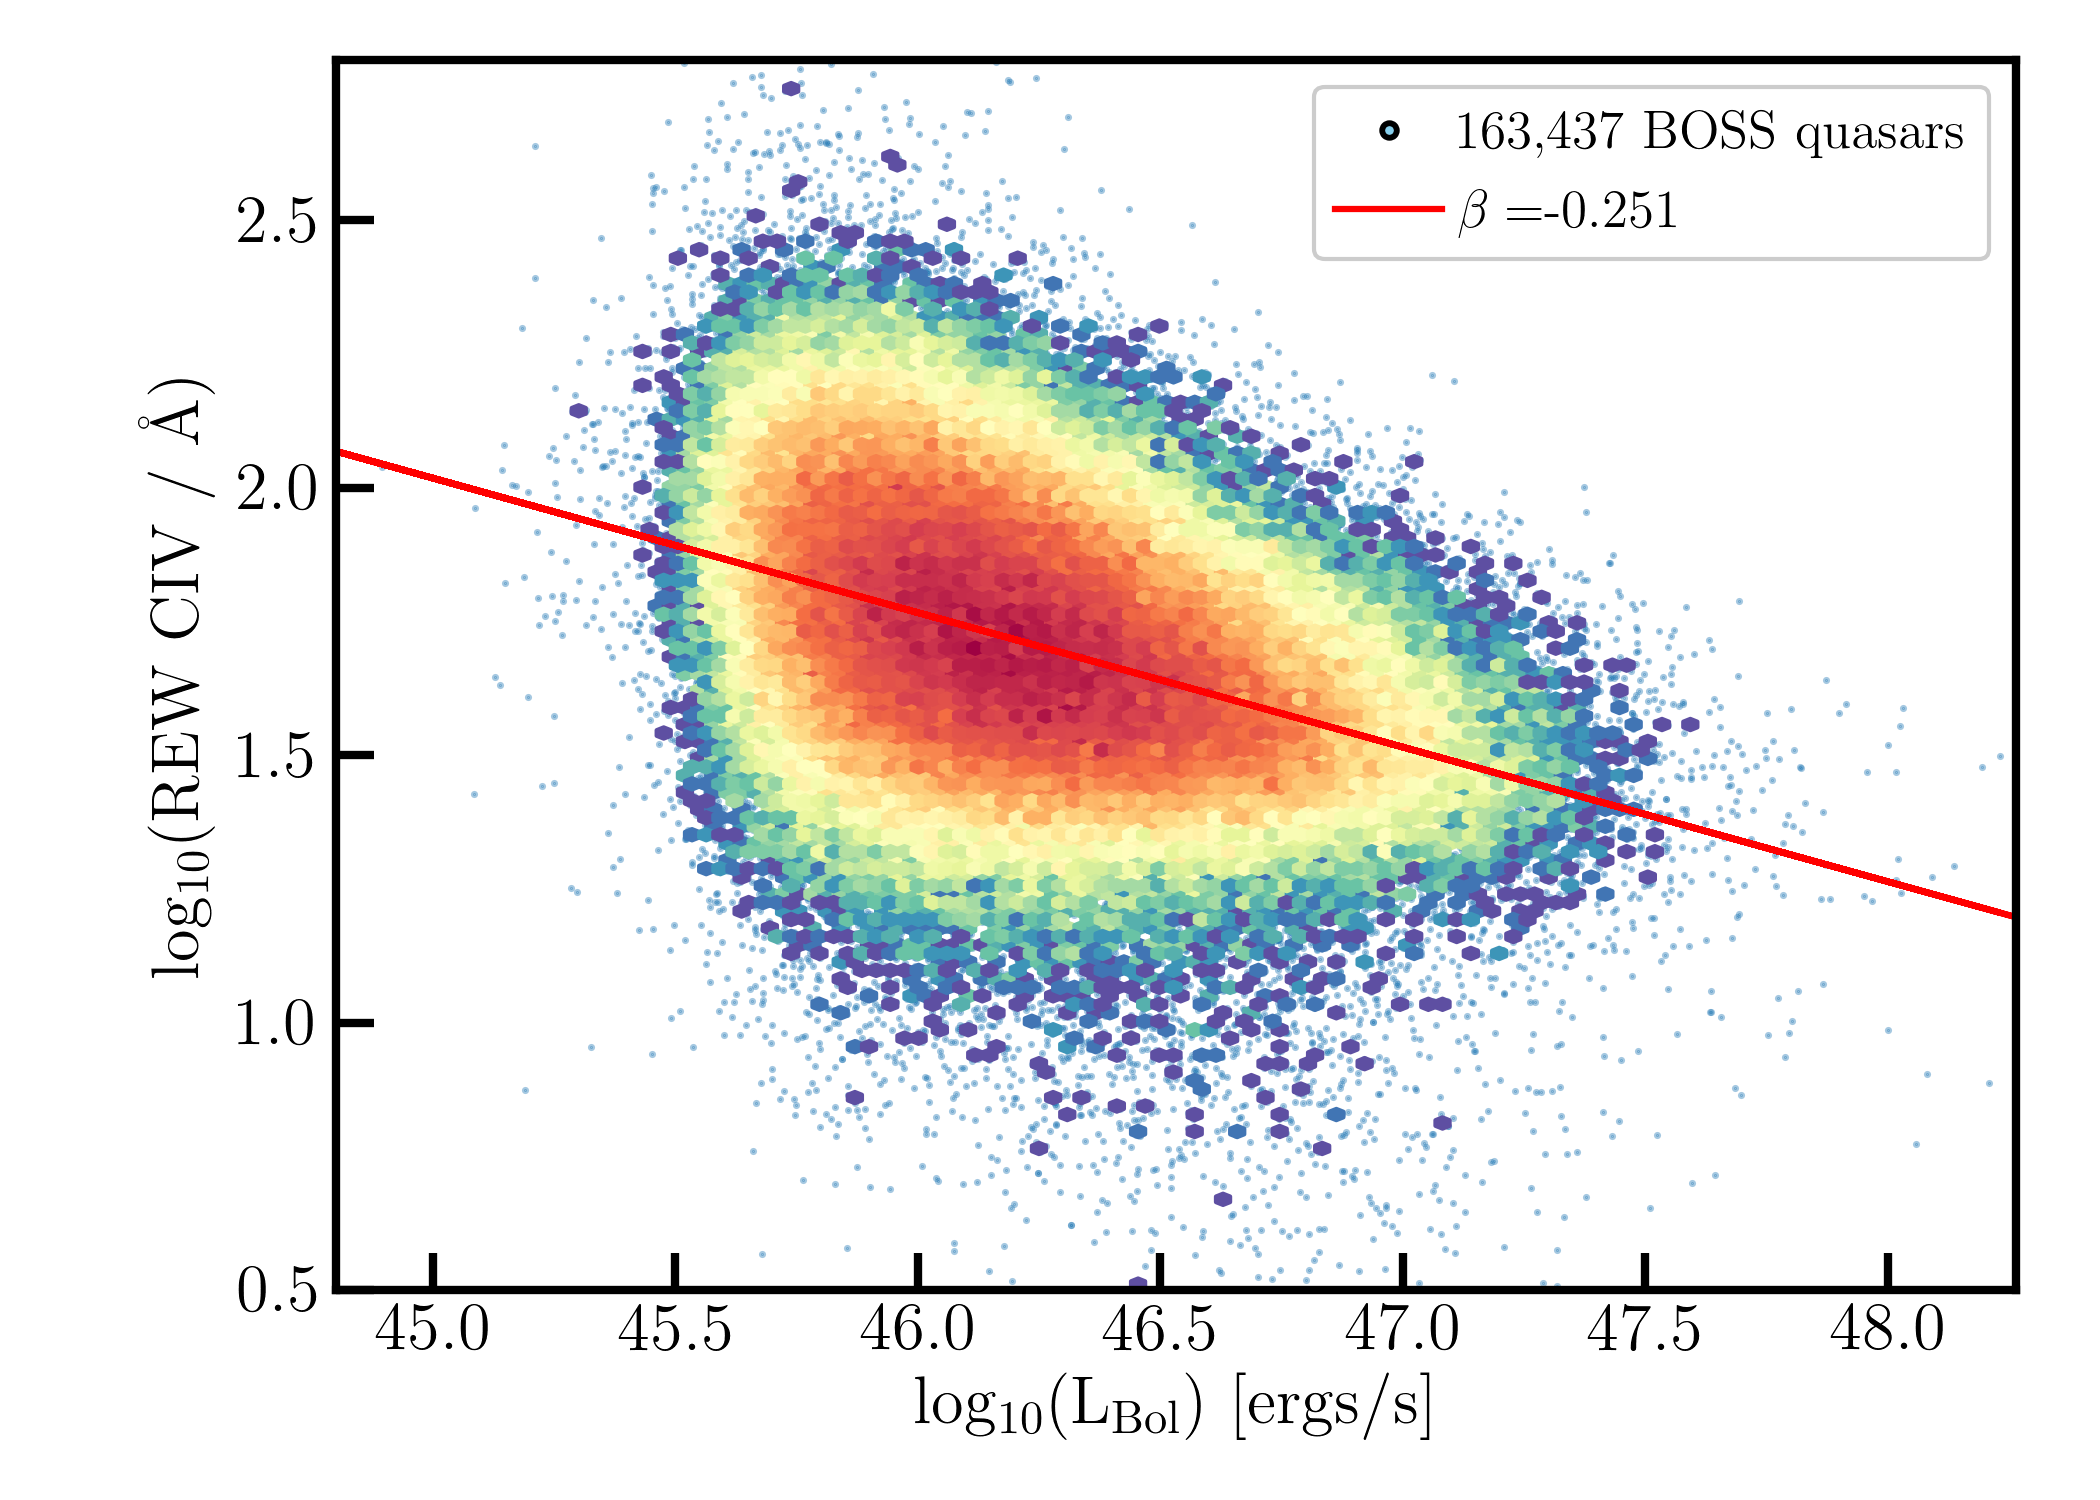
\includegraphics[width=8.7cm, trim=0.2cm 0.2cm 0.2cm 0.2cm, clip]
  {figures/CIV_CLQs_Baldwin_LBol_20191015.png}
   \vspace{-12pt}
   \caption[]{The Baldwin Plot. The bolometric luminosities are from \citet{Kozlowski2017},
     while the REW measurements are from \citet{Hamann2017}.}
  \label{fig:REWvsFWHM}
\end{figure}



\section{Conclusions}
In this paper we have reported on three redshift $z>2$ quasars with
dramatic changes in their \civ\ emission lines, the first
`Changing-Look'' quasars at high redshift.  This is also the first
time the changing-look behaviour has been seen in a high-ionization
emission line.

\begin{itemize}
  \item SDSS J1205+3422, J1638+2827 and J2228+2201 show interesting behaviour
in their observed optical light curves, and subsequent spectroscopy
shows significant changes in the \civ\ broad emission line, with both
line collapse and emergence being displayed in rest-frame timescales
of $\sim$240-1640 days.
\item Where observed, the profile of the Ly$\alpha$/\nv emission complex
also changes, and there is tentative evidence for changes in the \mgii
line.
\item Although line measurements from the three quasars show large changes
in the \civ\ line flux-line width plane, the quasars are not seen to
be outliers when considered against the full $z>2$ quasar population
in terms of (rest) Equivalent Width and FWHM properties.
\item 
We put these observations in context with recent ``state-change''
models, but note that even in their `low-state', the \civ\ CLQs are
above $\sim10\%$ in Eddington luminosity.
\end{itemize}

Etiam mollis viverra nisi eget aliquet. Aliquam erat volutpat. Vivamus
tristique, nisl eu malesuada semper, libero tortor convallis elit, a
scelerisque orci nisi lacinia turpis. In lacinia ultrices
volutpat. Proin ultrices luctus tellus, in placerat eros tincidunt
id. Ut varius iaculis quam in consequat. Nulla nec orci est, sit amet
Aliquam ac metus nec odio tempus pharetra sed nec diam. Sed eget arcu
nulla. Etiam elementum ultrices ligula, at iaculis libero feugiat
bibendum. Suspendisse potenti. Nam pharetra adipiscing
euismod. Quisque imperdiet dignissim odio, sed volutpat justo
tincidunt eu. Nunc vehicula pharetra suscipit. Integer aliquet pretium
ipsum vel ultrices. Nam rutrum nibh ac quam pulvinar molestie.



\subsection*{Availability of Data and computer analysis codes} 
All materials, databases, data tables and code are fully available at: 
\href{https://github.com/d80b2t/VHzQ}{\tt https://github.com/d80b2t/}


\section*{Acknowledgements}
NPR acknowledges support from the STFC and the Ernest Rutherford Fellowship scheme. 
%% KESF \& BM are supported by NSF PAARE AST-1153335. 
%% KESF \& BM thank CalTech/JPL for support during sabbatical.  

\noindent
We thank:
\begin{list}{$\circ$}{}  
  \item Andy Lawrence, Mike Hawkins and David Homan for useful discussion. 
\end{list}

This paper heavily used \href{http://www.star.bris.ac.uk/~mbt/topcat/}{TOPCAT} (v4.4)
\citep[][]{Taylor2005, Taylor2011}.
%%
This research made use of \href{http://www.astropy.org}{\tt Astropy}, 
a community-developed core Python package for Astronomy 
\citep{AstropyCollaboration2013, AstropyCollaboration2018}.

Funding for SDSS-III has been provided by the Alfred P. Sloan
Foundation, the Participating Institutions, the National Science
Foundation, and the U.S. Department of Energy Office of Science. The
SDSS-III web site is
\href{http://www.sdss3.org/}{http://www.sdss3.org/}.
%%
SDSS-III is managed by the Astrophysical Research Consortium for the
Participating Institutions of the SDSS-III Collaboration including the
University of Arizona, the Brazilian Participation Group, Brookhaven
National Laboratory, Carnegie Mellon University, University of
Florida, the French Participation Group, the German Participation
Group, Harvard University, the Instituto de Astrofisica de Canarias,
the Michigan State/Notre Dame/JINA Participation Group, Johns Hopkins
University, Lawrence Berkeley National Laboratory, Max Planck
Institute for Astrophysics, Max Planck Institute for Extraterrestrial
Physics, New Mexico State University, New York University, Ohio State
University, Pennsylvania State University, University of Portsmouth,
Princeton University, the Spanish Participation Group, University of
Tokyo, University of Utah, Vanderbilt University, University of
Virginia, University of Washington, and Yale University.

This publication makes use of data products from the Wide-field
Infrared Survey Explorer, which is a joint project of the University
of California, Los Angeles, and the Jet Propulsion
Laboratory/California Institute of Technology, and NEOWISE, which is a
project of the Jet Propulsion Laboratory/California Institute of
Technology. WISE and NEOWISE are funded by the National Aeronautics
and Space Administration. No animals were harmed in the production of
this paper, but there was a large spider in NPRs apartment that
``vanished''.

\bibliographystyle{mnras}
\bibliography{tester_mnras}


% Don't change these lines
\bsp	% typesetting comment
\label{lastpage}
\end{document}


\end{document}